\documentclass[twoside]{book}

% Packages required by doxygen
\usepackage{fixltx2e}
\usepackage{calc}
\usepackage{doxygen}
\usepackage[export]{adjustbox} % also loads graphicx
\usepackage{graphicx}
\usepackage[utf8]{inputenc}
\usepackage{makeidx}
\usepackage{multicol}
\usepackage{multirow}
\PassOptionsToPackage{warn}{textcomp}
\usepackage{textcomp}
\usepackage[nointegrals]{wasysym}
\usepackage[table]{xcolor}

% Font selection
\usepackage[T1]{fontenc}
\usepackage[scaled=.90]{helvet}
\usepackage{courier}
\usepackage{amssymb}
\usepackage{sectsty}
\renewcommand{\familydefault}{\sfdefault}
\allsectionsfont{%
  \fontseries{bc}\selectfont%
  \color{darkgray}%
}
\renewcommand{\DoxyLabelFont}{%
  \fontseries{bc}\selectfont%
  \color{darkgray}%
}
\newcommand{\+}{\discretionary{\mbox{\scriptsize$\hookleftarrow$}}{}{}}

% Page & text layout
\usepackage{geometry}
\geometry{%
  a4paper,%
  top=2.5cm,%
  bottom=2.5cm,%
  left=2.5cm,%
  right=2.5cm%
}
\tolerance=750
\hfuzz=15pt
\hbadness=750
\setlength{\emergencystretch}{15pt}
\setlength{\parindent}{0cm}
\setlength{\parskip}{3ex plus 2ex minus 2ex}
\makeatletter
\renewcommand{\paragraph}{%
  \@startsection{paragraph}{4}{0ex}{-1.0ex}{1.0ex}{%
    \normalfont\normalsize\bfseries\SS@parafont%
  }%
}
\renewcommand{\subparagraph}{%
  \@startsection{subparagraph}{5}{0ex}{-1.0ex}{1.0ex}{%
    \normalfont\normalsize\bfseries\SS@subparafont%
  }%
}
\makeatother

% Headers & footers
\usepackage{fancyhdr}
\pagestyle{fancyplain}
\fancyhead[LE]{\fancyplain{}{\bfseries\thepage}}
\fancyhead[CE]{\fancyplain{}{}}
\fancyhead[RE]{\fancyplain{}{\bfseries\leftmark}}
\fancyhead[LO]{\fancyplain{}{\bfseries\rightmark}}
\fancyhead[CO]{\fancyplain{}{}}
\fancyhead[RO]{\fancyplain{}{\bfseries\thepage}}
\fancyfoot[LE]{\fancyplain{}{}}
\fancyfoot[CE]{\fancyplain{}{}}
\fancyfoot[RE]{\fancyplain{}{\bfseries\scriptsize Generated by Doxygen }}
\fancyfoot[LO]{\fancyplain{}{\bfseries\scriptsize Generated by Doxygen }}
\fancyfoot[CO]{\fancyplain{}{}}
\fancyfoot[RO]{\fancyplain{}{}}
\renewcommand{\footrulewidth}{0.4pt}
\renewcommand{\chaptermark}[1]{%
  \markboth{#1}{}%
}
\renewcommand{\sectionmark}[1]{%
  \markright{\thesection\ #1}%
}

% Indices & bibliography
\usepackage{natbib}
\usepackage[titles]{tocloft}
\setcounter{tocdepth}{3}
\setcounter{secnumdepth}{5}
\makeindex

% Hyperlinks (required, but should be loaded last)
\usepackage{ifpdf}
\ifpdf
  \usepackage[pdftex,pagebackref=true]{hyperref}
\else
  \usepackage[ps2pdf,pagebackref=true]{hyperref}
\fi
\hypersetup{%
  colorlinks=true,%
  linkcolor=blue,%
  citecolor=blue,%
  unicode%
}

% Custom commands
\newcommand{\clearemptydoublepage}{%
  \newpage{\pagestyle{empty}\cleardoublepage}%
}

\usepackage{caption}
\captionsetup{labelsep=space,justification=centering,font={bf},singlelinecheck=off,skip=4pt,position=top}

%===== C O N T E N T S =====

\begin{document}

% Titlepage & ToC
\hypersetup{pageanchor=false,
             bookmarksnumbered=true,
             pdfencoding=unicode
            }
\pagenumbering{alph}
\begin{titlepage}
\vspace*{7cm}
\begin{center}%
{\Large enum robot \\[1ex]\large 1.\+0 }\\
\vspace*{1cm}
{\large Generated by Doxygen 1.8.13}\\
\end{center}
\end{titlepage}
\clearemptydoublepage
\pagenumbering{roman}
\tableofcontents
\clearemptydoublepage
\pagenumbering{arabic}
\hypersetup{pageanchor=true}

%--- Begin generated contents ---
\chapter{Example-\/\+Enum-\/\+Bot}
\label{md_README}
\Hypertarget{md_README}
\input{md_README}
\chapter{Namespace Index}
\section{Packages}
Here are the packages with brief descriptions (if available)\+:\begin{DoxyCompactList}
\item\contentsline{section}{\hyperlink{namespacefrc}{frc} }{\pageref{namespacefrc}}{}
\item\contentsline{section}{\hyperlink{namespacefrc_1_1robot}{frc.\+robot} }{\pageref{namespacefrc_1_1robot}}{}
\item\contentsline{section}{\hyperlink{namespacefrc_1_1robot_1_1_enums}{frc.\+robot.\+Enums} }{\pageref{namespacefrc_1_1robot_1_1_enums}}{}
\item\contentsline{section}{\hyperlink{namespacefrc_1_1robot_1_1subsystems}{frc.\+robot.\+subsystems} }{\pageref{namespacefrc_1_1robot_1_1subsystems}}{}
\end{DoxyCompactList}

\chapter{Hierarchical Index}
\section{Class Hierarchy}
This inheritance list is sorted roughly, but not completely, alphabetically\+:\begin{DoxyCompactList}
\item \contentsline{section}{frc.\+robot.\+subsystems.\+Cargo}{\pageref{classfrc_1_1robot_1_1subsystems_1_1_cargo}}{}
\item \contentsline{section}{frc.\+robot.\+subsystems.\+Drive\+Train}{\pageref{classfrc_1_1robot_1_1subsystems_1_1_drive_train}}{}
\item \contentsline{section}{frc.\+robot.\+Enums.\+Hatch}{\pageref{enumfrc_1_1robot_1_1_enums_1_1_hatch}}{}
\item \contentsline{section}{frc.\+robot.\+subsystems.\+Hatch\+\_\+\+Control}{\pageref{classfrc_1_1robot_1_1subsystems_1_1_hatch___control}}{}
\item \contentsline{section}{frc.\+robot.\+Enums.\+Lift\+\_\+\+Pistons}{\pageref{enumfrc_1_1robot_1_1_enums_1_1_lift___pistons}}{}
\item \contentsline{section}{frc.\+robot.\+Main}{\pageref{classfrc_1_1robot_1_1_main}}{}
\item \contentsline{section}{frc.\+robot.\+OI}{\pageref{classfrc_1_1robot_1_1_o_i}}{}
\item \contentsline{section}{frc.\+robot.\+Robot\+Map}{\pageref{classfrc_1_1robot_1_1_robot_map}}{}
\item \contentsline{section}{frc.\+robot.\+Enums.\+Shift}{\pageref{enumfrc_1_1robot_1_1_enums_1_1_shift}}{}
\item \contentsline{section}{frc.\+robot.\+subsystems.\+Stilts}{\pageref{classfrc_1_1robot_1_1subsystems_1_1_stilts}}{}
\item \contentsline{section}{frc.\+robot.\+subsystems.\+Teleop}{\pageref{classfrc_1_1robot_1_1subsystems_1_1_teleop}}{}
\item \contentsline{section}{frc.\+robot.\+subsystems.\+Teleop\+\_\+\+Controller2}{\pageref{classfrc_1_1robot_1_1subsystems_1_1_teleop___controller2}}{}
\item Timed\+Robot\begin{DoxyCompactList}
\item \contentsline{section}{frc.\+robot.\+Robot}{\pageref{classfrc_1_1robot_1_1_robot}}{}
\end{DoxyCompactList}
\end{DoxyCompactList}

\chapter{Class Index}
\section{Class List}
Here are the classes, structs, unions and interfaces with brief descriptions\+:\begin{DoxyCompactList}
\item\contentsline{section}{\hyperlink{classfrc_1_1robot_1_1subsystems_1_1_cargo}{frc.\+robot.\+subsystems.\+Cargo} }{\pageref{classfrc_1_1robot_1_1subsystems_1_1_cargo}}{}
\item\contentsline{section}{\hyperlink{classfrc_1_1robot_1_1subsystems_1_1_drive_train}{frc.\+robot.\+subsystems.\+Drive\+Train} }{\pageref{classfrc_1_1robot_1_1subsystems_1_1_drive_train}}{}
\item\contentsline{section}{\hyperlink{enumfrc_1_1robot_1_1_enums_1_1_hatch}{frc.\+robot.\+Enums.\+Hatch} }{\pageref{enumfrc_1_1robot_1_1_enums_1_1_hatch}}{}
\item\contentsline{section}{\hyperlink{classfrc_1_1robot_1_1subsystems_1_1_hatch___control}{frc.\+robot.\+subsystems.\+Hatch\+\_\+\+Control} }{\pageref{classfrc_1_1robot_1_1subsystems_1_1_hatch___control}}{}
\item\contentsline{section}{\hyperlink{enumfrc_1_1robot_1_1_enums_1_1_lift___pistons}{frc.\+robot.\+Enums.\+Lift\+\_\+\+Pistons} }{\pageref{enumfrc_1_1robot_1_1_enums_1_1_lift___pistons}}{}
\item\contentsline{section}{\hyperlink{classfrc_1_1robot_1_1_main}{frc.\+robot.\+Main} \\*Do N\+OT add any static variables to this class, or any initialization at all }{\pageref{classfrc_1_1robot_1_1_main}}{}
\item\contentsline{section}{\hyperlink{classfrc_1_1robot_1_1_o_i}{frc.\+robot.\+OI} \\*This class is the glue that binds the controls on the physical operator interface to the commands and command groups that allow control of the robot }{\pageref{classfrc_1_1robot_1_1_o_i}}{}
\item\contentsline{section}{\hyperlink{classfrc_1_1robot_1_1_robot}{frc.\+robot.\+Robot} }{\pageref{classfrc_1_1robot_1_1_robot}}{}
\item\contentsline{section}{\hyperlink{classfrc_1_1robot_1_1_robot_map}{frc.\+robot.\+Robot\+Map} \\*The \hyperlink{classfrc_1_1robot_1_1_robot_map}{Robot\+Map} is a mapping from the ports sensors and actuators are wired into to a variable name }{\pageref{classfrc_1_1robot_1_1_robot_map}}{}
\item\contentsline{section}{\hyperlink{enumfrc_1_1robot_1_1_enums_1_1_shift}{frc.\+robot.\+Enums.\+Shift} }{\pageref{enumfrc_1_1robot_1_1_enums_1_1_shift}}{}
\item\contentsline{section}{\hyperlink{classfrc_1_1robot_1_1subsystems_1_1_stilts}{frc.\+robot.\+subsystems.\+Stilts} }{\pageref{classfrc_1_1robot_1_1subsystems_1_1_stilts}}{}
\item\contentsline{section}{\hyperlink{classfrc_1_1robot_1_1subsystems_1_1_teleop}{frc.\+robot.\+subsystems.\+Teleop} }{\pageref{classfrc_1_1robot_1_1subsystems_1_1_teleop}}{}
\item\contentsline{section}{\hyperlink{classfrc_1_1robot_1_1subsystems_1_1_teleop___controller2}{frc.\+robot.\+subsystems.\+Teleop\+\_\+\+Controller2} }{\pageref{classfrc_1_1robot_1_1subsystems_1_1_teleop___controller2}}{}
\end{DoxyCompactList}

\chapter{File Index}
\section{File List}
Here is a list of all files with brief descriptions\+:\begin{DoxyCompactList}
\item\contentsline{section}{src/main/java/frc/robot/\hyperlink{_main_8java}{Main.\+java} }{\pageref{_main_8java}}{}
\item\contentsline{section}{src/main/java/frc/robot/\hyperlink{_o_i_8java}{O\+I.\+java} }{\pageref{_o_i_8java}}{}
\item\contentsline{section}{src/main/java/frc/robot/\hyperlink{_robot_8java}{Robot.\+java} }{\pageref{_robot_8java}}{}
\item\contentsline{section}{src/main/java/frc/robot/\hyperlink{_robot_map_8java}{Robot\+Map.\+java} }{\pageref{_robot_map_8java}}{}
\item\contentsline{section}{src/main/java/frc/robot/\+Enums/\hyperlink{_hatch_8java}{Hatch.\+java} }{\pageref{_hatch_8java}}{}
\item\contentsline{section}{src/main/java/frc/robot/\+Enums/\hyperlink{_lift___pistons_8java}{Lift\+\_\+\+Pistons.\+java} }{\pageref{_lift___pistons_8java}}{}
\item\contentsline{section}{src/main/java/frc/robot/\+Enums/\hyperlink{_shift_8java}{Shift.\+java} }{\pageref{_shift_8java}}{}
\item\contentsline{section}{src/main/java/frc/robot/subsystems/\hyperlink{_cargo_8java}{Cargo.\+java} }{\pageref{_cargo_8java}}{}
\item\contentsline{section}{src/main/java/frc/robot/subsystems/\hyperlink{_drive_train_8java}{Drive\+Train.\+java} }{\pageref{_drive_train_8java}}{}
\item\contentsline{section}{src/main/java/frc/robot/subsystems/\hyperlink{_hatch___control_8java}{Hatch\+\_\+\+Control.\+java} }{\pageref{_hatch___control_8java}}{}
\item\contentsline{section}{src/main/java/frc/robot/subsystems/\hyperlink{_stilts_8java}{Stilts.\+java} }{\pageref{_stilts_8java}}{}
\item\contentsline{section}{src/main/java/frc/robot/subsystems/\hyperlink{_teleop_8java}{Teleop.\+java} }{\pageref{_teleop_8java}}{}
\item\contentsline{section}{src/main/java/frc/robot/subsystems/\hyperlink{_teleop___controller2_8java}{Teleop\+\_\+\+Controller2.\+java} }{\pageref{_teleop___controller2_8java}}{}
\end{DoxyCompactList}

\chapter{Namespace Documentation}
\hypertarget{namespacefrc}{}\section{Package frc}
\label{namespacefrc}\index{frc@{frc}}
\subsection*{Packages}
\begin{DoxyCompactItemize}
\item 
package \hyperlink{namespacefrc_1_1robot}{robot}
\end{DoxyCompactItemize}

\hypertarget{namespacefrc_1_1robot}{}\section{Package frc.\+robot}
\label{namespacefrc_1_1robot}\index{frc.\+robot@{frc.\+robot}}
\subsection*{Packages}
\begin{DoxyCompactItemize}
\item 
package \hyperlink{namespacefrc_1_1robot_1_1Enums}{Enums}
\item 
package \hyperlink{namespacefrc_1_1robot_1_1subsystems}{subsystems}
\end{DoxyCompactItemize}
\subsection*{Classes}
\begin{DoxyCompactItemize}
\item 
class \hyperlink{classfrc_1_1robot_1_1Main}{Main}
\begin{DoxyCompactList}\small\item\em Do N\+OT add any static variables to this class, or any initialization at all. \end{DoxyCompactList}\item 
class \hyperlink{classfrc_1_1robot_1_1OI}{OI}
\begin{DoxyCompactList}\small\item\em This class is the glue that binds the controls on the physical operator interface to the commands and command groups that allow control of the robot. \end{DoxyCompactList}\item 
class \hyperlink{classfrc_1_1robot_1_1Robot}{Robot}
\item 
class \hyperlink{classfrc_1_1robot_1_1RobotMap}{Robot\+Map}
\begin{DoxyCompactList}\small\item\em The \hyperlink{classfrc_1_1robot_1_1RobotMap}{Robot\+Map} is a mapping from the ports sensors and actuators are wired into to a variable name. \end{DoxyCompactList}\end{DoxyCompactItemize}

\hypertarget{namespacefrc_1_1robot_1_1Enums}{}\section{Package frc.\+robot.\+Enums}
\label{namespacefrc_1_1robot_1_1Enums}\index{frc.\+robot.\+Enums@{frc.\+robot.\+Enums}}
\subsection*{Classes}
\begin{DoxyCompactItemize}
\item 
enum \hyperlink{enumfrc_1_1robot_1_1Enums_1_1Hatch}{Hatch}
\item 
enum \hyperlink{enumfrc_1_1robot_1_1Enums_1_1Lift__Pistons}{Lift\+\_\+\+Pistons}
\item 
enum \hyperlink{enumfrc_1_1robot_1_1Enums_1_1Shift}{Shift}
\end{DoxyCompactItemize}

\hypertarget{namespacefrc_1_1robot_1_1subsystems}{}\section{Package frc.\+robot.\+subsystems}
\label{namespacefrc_1_1robot_1_1subsystems}\index{frc.\+robot.\+subsystems@{frc.\+robot.\+subsystems}}
\subsection*{Classes}
\begin{DoxyCompactItemize}
\item 
class \hyperlink{classfrc_1_1robot_1_1subsystems_1_1Cargo}{Cargo}
\item 
class \hyperlink{classfrc_1_1robot_1_1subsystems_1_1DriveTrain}{Drive\+Train}
\item 
class \hyperlink{classfrc_1_1robot_1_1subsystems_1_1Hatch__Control}{Hatch\+\_\+\+Control}
\item 
class \hyperlink{classfrc_1_1robot_1_1subsystems_1_1Stilts}{Stilts}
\item 
class \hyperlink{classfrc_1_1robot_1_1subsystems_1_1Teleop}{Teleop}
\item 
class \hyperlink{classfrc_1_1robot_1_1subsystems_1_1Teleop__Controller2}{Teleop\+\_\+\+Controller2}
\end{DoxyCompactItemize}

\chapter{Class Documentation}
\hypertarget{classfrc_1_1robot_1_1subsystems_1_1Cargo}{}\section{frc.\+robot.\+subsystems.\+Cargo Class Reference}
\label{classfrc_1_1robot_1_1subsystems_1_1Cargo}\index{frc.\+robot.\+subsystems.\+Cargo@{frc.\+robot.\+subsystems.\+Cargo}}


Collaboration diagram for frc.\+robot.\+subsystems.\+Cargo\+:\nopagebreak
\begin{figure}[H]
\begin{center}
\leavevmode
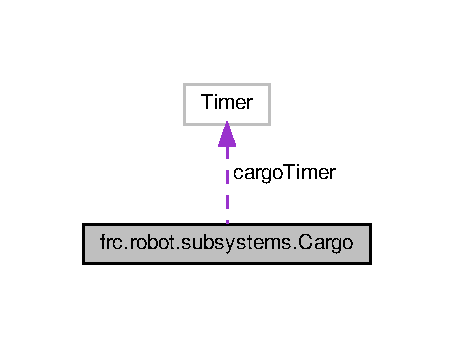
\includegraphics[width=218pt]{classfrc_1_1robot_1_1subsystems_1_1Cargo__coll__graph}
\end{center}
\end{figure}
\subsection*{Public Member Functions}
\begin{DoxyCompactItemize}
\item 
\hyperlink{classfrc_1_1robot_1_1subsystems_1_1Cargo_ad27213bb1c8c9a33d5c2b9cc153c1508}{Cargo} ()
\end{DoxyCompactItemize}
\subsection*{Static Public Member Functions}
\begin{DoxyCompactItemize}
\item 
static void \hyperlink{classfrc_1_1robot_1_1subsystems_1_1Cargo_aa8640bc75e8b3f2472ea586936d6ed1f}{actuate\+Arm} (double speed)
\item 
static void \hyperlink{classfrc_1_1robot_1_1subsystems_1_1Cargo_aa85a0b3aa7cb498f4b1c7eac6d26bce2}{stop\+Arm} ()
\item 
static void \hyperlink{classfrc_1_1robot_1_1subsystems_1_1Cargo_aa05df516e815067a7b853d9fbdc35f01}{actuate\+Claw} (double speed)
\item 
static void \hyperlink{classfrc_1_1robot_1_1subsystems_1_1Cargo_a0ac97ff2fa2f7af96744a5dcba7ba61b}{stop\+Claw} ()
\item 
static void \hyperlink{classfrc_1_1robot_1_1subsystems_1_1Cargo_a8a4dd09c62967c4d82af8953cf8ab731}{hold\+Ball} ()
\item 
static void \hyperlink{classfrc_1_1robot_1_1subsystems_1_1Cargo_a20e8230acdc07d7d94e056f9e09d91ad}{update} ()
\end{DoxyCompactItemize}
\subsection*{Static Public Attributes}
\begin{DoxyCompactItemize}
\item 
static Timer \hyperlink{classfrc_1_1robot_1_1subsystems_1_1Cargo_a50722902fa0c3ad0db5f592ad51b94f6}{cargo\+Timer} = new Timer()
\end{DoxyCompactItemize}


\subsection{Detailed Description}


Definition at line 7 of file Cargo.\+java.



\subsection{Constructor \& Destructor Documentation}
\mbox{\Hypertarget{classfrc_1_1robot_1_1subsystems_1_1Cargo_ad27213bb1c8c9a33d5c2b9cc153c1508}\label{classfrc_1_1robot_1_1subsystems_1_1Cargo_ad27213bb1c8c9a33d5c2b9cc153c1508}} 
\index{frc\+::robot\+::subsystems\+::\+Cargo@{frc\+::robot\+::subsystems\+::\+Cargo}!Cargo@{Cargo}}
\index{Cargo@{Cargo}!frc\+::robot\+::subsystems\+::\+Cargo@{frc\+::robot\+::subsystems\+::\+Cargo}}
\subsubsection{\texorpdfstring{Cargo()}{Cargo()}}
{\footnotesize\ttfamily frc.\+robot.\+subsystems.\+Cargo.\+Cargo (\begin{DoxyParamCaption}{ }\end{DoxyParamCaption})}



Definition at line 13 of file Cargo.\+java.



\subsection{Member Function Documentation}
\mbox{\Hypertarget{classfrc_1_1robot_1_1subsystems_1_1Cargo_aa8640bc75e8b3f2472ea586936d6ed1f}\label{classfrc_1_1robot_1_1subsystems_1_1Cargo_aa8640bc75e8b3f2472ea586936d6ed1f}} 
\index{frc\+::robot\+::subsystems\+::\+Cargo@{frc\+::robot\+::subsystems\+::\+Cargo}!actuate\+Arm@{actuate\+Arm}}
\index{actuate\+Arm@{actuate\+Arm}!frc\+::robot\+::subsystems\+::\+Cargo@{frc\+::robot\+::subsystems\+::\+Cargo}}
\subsubsection{\texorpdfstring{actuate\+Arm()}{actuateArm()}}
{\footnotesize\ttfamily static void frc.\+robot.\+subsystems.\+Cargo.\+actuate\+Arm (\begin{DoxyParamCaption}\item[{double}]{speed }\end{DoxyParamCaption})\hspace{0.3cm}{\ttfamily [static]}}



Definition at line 14 of file Cargo.\+java.

\mbox{\Hypertarget{classfrc_1_1robot_1_1subsystems_1_1Cargo_aa05df516e815067a7b853d9fbdc35f01}\label{classfrc_1_1robot_1_1subsystems_1_1Cargo_aa05df516e815067a7b853d9fbdc35f01}} 
\index{frc\+::robot\+::subsystems\+::\+Cargo@{frc\+::robot\+::subsystems\+::\+Cargo}!actuate\+Claw@{actuate\+Claw}}
\index{actuate\+Claw@{actuate\+Claw}!frc\+::robot\+::subsystems\+::\+Cargo@{frc\+::robot\+::subsystems\+::\+Cargo}}
\subsubsection{\texorpdfstring{actuate\+Claw()}{actuateClaw()}}
{\footnotesize\ttfamily static void frc.\+robot.\+subsystems.\+Cargo.\+actuate\+Claw (\begin{DoxyParamCaption}\item[{double}]{speed }\end{DoxyParamCaption})\hspace{0.3cm}{\ttfamily [static]}}



Definition at line 20 of file Cargo.\+java.

\mbox{\Hypertarget{classfrc_1_1robot_1_1subsystems_1_1Cargo_a8a4dd09c62967c4d82af8953cf8ab731}\label{classfrc_1_1robot_1_1subsystems_1_1Cargo_a8a4dd09c62967c4d82af8953cf8ab731}} 
\index{frc\+::robot\+::subsystems\+::\+Cargo@{frc\+::robot\+::subsystems\+::\+Cargo}!hold\+Ball@{hold\+Ball}}
\index{hold\+Ball@{hold\+Ball}!frc\+::robot\+::subsystems\+::\+Cargo@{frc\+::robot\+::subsystems\+::\+Cargo}}
\subsubsection{\texorpdfstring{hold\+Ball()}{holdBall()}}
{\footnotesize\ttfamily static void frc.\+robot.\+subsystems.\+Cargo.\+hold\+Ball (\begin{DoxyParamCaption}{ }\end{DoxyParamCaption})\hspace{0.3cm}{\ttfamily [static]}}



Definition at line 26 of file Cargo.\+java.

\mbox{\Hypertarget{classfrc_1_1robot_1_1subsystems_1_1Cargo_aa85a0b3aa7cb498f4b1c7eac6d26bce2}\label{classfrc_1_1robot_1_1subsystems_1_1Cargo_aa85a0b3aa7cb498f4b1c7eac6d26bce2}} 
\index{frc\+::robot\+::subsystems\+::\+Cargo@{frc\+::robot\+::subsystems\+::\+Cargo}!stop\+Arm@{stop\+Arm}}
\index{stop\+Arm@{stop\+Arm}!frc\+::robot\+::subsystems\+::\+Cargo@{frc\+::robot\+::subsystems\+::\+Cargo}}
\subsubsection{\texorpdfstring{stop\+Arm()}{stopArm()}}
{\footnotesize\ttfamily static void frc.\+robot.\+subsystems.\+Cargo.\+stop\+Arm (\begin{DoxyParamCaption}{ }\end{DoxyParamCaption})\hspace{0.3cm}{\ttfamily [static]}}



Definition at line 17 of file Cargo.\+java.

\mbox{\Hypertarget{classfrc_1_1robot_1_1subsystems_1_1Cargo_a0ac97ff2fa2f7af96744a5dcba7ba61b}\label{classfrc_1_1robot_1_1subsystems_1_1Cargo_a0ac97ff2fa2f7af96744a5dcba7ba61b}} 
\index{frc\+::robot\+::subsystems\+::\+Cargo@{frc\+::robot\+::subsystems\+::\+Cargo}!stop\+Claw@{stop\+Claw}}
\index{stop\+Claw@{stop\+Claw}!frc\+::robot\+::subsystems\+::\+Cargo@{frc\+::robot\+::subsystems\+::\+Cargo}}
\subsubsection{\texorpdfstring{stop\+Claw()}{stopClaw()}}
{\footnotesize\ttfamily static void frc.\+robot.\+subsystems.\+Cargo.\+stop\+Claw (\begin{DoxyParamCaption}{ }\end{DoxyParamCaption})\hspace{0.3cm}{\ttfamily [static]}}



Definition at line 23 of file Cargo.\+java.

\mbox{\Hypertarget{classfrc_1_1robot_1_1subsystems_1_1Cargo_a20e8230acdc07d7d94e056f9e09d91ad}\label{classfrc_1_1robot_1_1subsystems_1_1Cargo_a20e8230acdc07d7d94e056f9e09d91ad}} 
\index{frc\+::robot\+::subsystems\+::\+Cargo@{frc\+::robot\+::subsystems\+::\+Cargo}!update@{update}}
\index{update@{update}!frc\+::robot\+::subsystems\+::\+Cargo@{frc\+::robot\+::subsystems\+::\+Cargo}}
\subsubsection{\texorpdfstring{update()}{update()}}
{\footnotesize\ttfamily static void frc.\+robot.\+subsystems.\+Cargo.\+update (\begin{DoxyParamCaption}{ }\end{DoxyParamCaption})\hspace{0.3cm}{\ttfamily [static]}}



Definition at line 29 of file Cargo.\+java.



\subsection{Member Data Documentation}
\mbox{\Hypertarget{classfrc_1_1robot_1_1subsystems_1_1Cargo_a50722902fa0c3ad0db5f592ad51b94f6}\label{classfrc_1_1robot_1_1subsystems_1_1Cargo_a50722902fa0c3ad0db5f592ad51b94f6}} 
\index{frc\+::robot\+::subsystems\+::\+Cargo@{frc\+::robot\+::subsystems\+::\+Cargo}!cargo\+Timer@{cargo\+Timer}}
\index{cargo\+Timer@{cargo\+Timer}!frc\+::robot\+::subsystems\+::\+Cargo@{frc\+::robot\+::subsystems\+::\+Cargo}}
\subsubsection{\texorpdfstring{cargo\+Timer}{cargoTimer}}
{\footnotesize\ttfamily Timer frc.\+robot.\+subsystems.\+Cargo.\+cargo\+Timer = new Timer()\hspace{0.3cm}{\ttfamily [static]}}



Definition at line 8 of file Cargo.\+java.



The documentation for this class was generated from the following file\+:\begin{DoxyCompactItemize}
\item 
src/main/java/frc/robot/subsystems/\hyperlink{Cargo_8java}{Cargo.\+java}\end{DoxyCompactItemize}

\hypertarget{classfrc_1_1robot_1_1subsystems_1_1DriveTrain}{}\section{frc.\+robot.\+subsystems.\+Drive\+Train Class Reference}
\label{classfrc_1_1robot_1_1subsystems_1_1DriveTrain}\index{frc.\+robot.\+subsystems.\+Drive\+Train@{frc.\+robot.\+subsystems.\+Drive\+Train}}
\subsection*{Public Member Functions}
\begin{DoxyCompactItemize}
\item 
\hyperlink{classfrc_1_1robot_1_1subsystems_1_1DriveTrain_a39f30717e8df92af73d57c01ac0525df}{Drive\+Train} ()
\end{DoxyCompactItemize}
\subsection*{Static Public Member Functions}
\begin{DoxyCompactItemize}
\item 
static void \hyperlink{classfrc_1_1robot_1_1subsystems_1_1DriveTrain_a3288b5af8182d08f76290b257041538c}{shift} (\hyperlink{enumfrc_1_1robot_1_1Enums_1_1Shift}{Shift} direction)
\item 
static void \hyperlink{classfrc_1_1robot_1_1subsystems_1_1DriveTrain_a883baac3715e22887c0ec5ce825fbfab}{periodic} ()
\end{DoxyCompactItemize}


\subsection{Detailed Description}


Definition at line 10 of file Drive\+Train.\+java.



\subsection{Constructor \& Destructor Documentation}
\mbox{\Hypertarget{classfrc_1_1robot_1_1subsystems_1_1DriveTrain_a39f30717e8df92af73d57c01ac0525df}\label{classfrc_1_1robot_1_1subsystems_1_1DriveTrain_a39f30717e8df92af73d57c01ac0525df}} 
\index{frc\+::robot\+::subsystems\+::\+Drive\+Train@{frc\+::robot\+::subsystems\+::\+Drive\+Train}!Drive\+Train@{Drive\+Train}}
\index{Drive\+Train@{Drive\+Train}!frc\+::robot\+::subsystems\+::\+Drive\+Train@{frc\+::robot\+::subsystems\+::\+Drive\+Train}}
\subsubsection{\texorpdfstring{Drive\+Train()}{DriveTrain()}}
{\footnotesize\ttfamily frc.\+robot.\+subsystems.\+Drive\+Train.\+Drive\+Train (\begin{DoxyParamCaption}{ }\end{DoxyParamCaption})}



Definition at line 12 of file Drive\+Train.\+java.



\subsection{Member Function Documentation}
\mbox{\Hypertarget{classfrc_1_1robot_1_1subsystems_1_1DriveTrain_a883baac3715e22887c0ec5ce825fbfab}\label{classfrc_1_1robot_1_1subsystems_1_1DriveTrain_a883baac3715e22887c0ec5ce825fbfab}} 
\index{frc\+::robot\+::subsystems\+::\+Drive\+Train@{frc\+::robot\+::subsystems\+::\+Drive\+Train}!periodic@{periodic}}
\index{periodic@{periodic}!frc\+::robot\+::subsystems\+::\+Drive\+Train@{frc\+::robot\+::subsystems\+::\+Drive\+Train}}
\subsubsection{\texorpdfstring{periodic()}{periodic()}}
{\footnotesize\ttfamily static void frc.\+robot.\+subsystems.\+Drive\+Train.\+periodic (\begin{DoxyParamCaption}{ }\end{DoxyParamCaption})\hspace{0.3cm}{\ttfamily [static]}}



Definition at line 28 of file Drive\+Train.\+java.

\mbox{\Hypertarget{classfrc_1_1robot_1_1subsystems_1_1DriveTrain_a3288b5af8182d08f76290b257041538c}\label{classfrc_1_1robot_1_1subsystems_1_1DriveTrain_a3288b5af8182d08f76290b257041538c}} 
\index{frc\+::robot\+::subsystems\+::\+Drive\+Train@{frc\+::robot\+::subsystems\+::\+Drive\+Train}!shift@{shift}}
\index{shift@{shift}!frc\+::robot\+::subsystems\+::\+Drive\+Train@{frc\+::robot\+::subsystems\+::\+Drive\+Train}}
\subsubsection{\texorpdfstring{shift()}{shift()}}
{\footnotesize\ttfamily static void frc.\+robot.\+subsystems.\+Drive\+Train.\+shift (\begin{DoxyParamCaption}\item[{\hyperlink{enumfrc_1_1robot_1_1Enums_1_1Shift}{Shift}}]{direction }\end{DoxyParamCaption})\hspace{0.3cm}{\ttfamily [static]}}



Definition at line 15 of file Drive\+Train.\+java.



The documentation for this class was generated from the following file\+:\begin{DoxyCompactItemize}
\item 
src/main/java/frc/robot/subsystems/\hyperlink{DriveTrain_8java}{Drive\+Train.\+java}\end{DoxyCompactItemize}

\hypertarget{enumfrc_1_1robot_1_1Enums_1_1Hatch}{}\section{frc.\+robot.\+Enums.\+Hatch Enum Reference}
\label{enumfrc_1_1robot_1_1Enums_1_1Hatch}\index{frc.\+robot.\+Enums.\+Hatch@{frc.\+robot.\+Enums.\+Hatch}}
\subsection*{Public Attributes}
\begin{DoxyCompactItemize}
\item 
\hyperlink{enumfrc_1_1robot_1_1Enums_1_1Hatch_aa9182f52be77e783bb38e7cfbf5bb700}{Extend}
\item 
\hyperlink{enumfrc_1_1robot_1_1Enums_1_1Hatch_ac4881a7e4ca2bc7c64aa8acd0da91d6e}{Retract}
\item 
\hyperlink{enumfrc_1_1robot_1_1Enums_1_1Hatch_aba378e125bbd0e4206aa27ab9bc51b0b}{Open}
\item 
\hyperlink{enumfrc_1_1robot_1_1Enums_1_1Hatch_ad9de6151d633f63ba3cb50aaeba1afd0}{Close}
\end{DoxyCompactItemize}


\subsection{Detailed Description}


Definition at line 4 of file Hatch.\+java.



\subsection{Member Data Documentation}
\mbox{\Hypertarget{enumfrc_1_1robot_1_1Enums_1_1Hatch_ad9de6151d633f63ba3cb50aaeba1afd0}\label{enumfrc_1_1robot_1_1Enums_1_1Hatch_ad9de6151d633f63ba3cb50aaeba1afd0}} 
\index{frc\+::robot\+::\+Enums\+::\+Hatch@{frc\+::robot\+::\+Enums\+::\+Hatch}!Close@{Close}}
\index{Close@{Close}!frc\+::robot\+::\+Enums\+::\+Hatch@{frc\+::robot\+::\+Enums\+::\+Hatch}}
\subsubsection{\texorpdfstring{Close}{Close}}
{\footnotesize\ttfamily frc.\+robot.\+Enums.\+Hatch.\+Close}



Definition at line 8 of file Hatch.\+java.

\mbox{\Hypertarget{enumfrc_1_1robot_1_1Enums_1_1Hatch_aa9182f52be77e783bb38e7cfbf5bb700}\label{enumfrc_1_1robot_1_1Enums_1_1Hatch_aa9182f52be77e783bb38e7cfbf5bb700}} 
\index{frc\+::robot\+::\+Enums\+::\+Hatch@{frc\+::robot\+::\+Enums\+::\+Hatch}!Extend@{Extend}}
\index{Extend@{Extend}!frc\+::robot\+::\+Enums\+::\+Hatch@{frc\+::robot\+::\+Enums\+::\+Hatch}}
\subsubsection{\texorpdfstring{Extend}{Extend}}
{\footnotesize\ttfamily frc.\+robot.\+Enums.\+Hatch.\+Extend}



Definition at line 5 of file Hatch.\+java.

\mbox{\Hypertarget{enumfrc_1_1robot_1_1Enums_1_1Hatch_aba378e125bbd0e4206aa27ab9bc51b0b}\label{enumfrc_1_1robot_1_1Enums_1_1Hatch_aba378e125bbd0e4206aa27ab9bc51b0b}} 
\index{frc\+::robot\+::\+Enums\+::\+Hatch@{frc\+::robot\+::\+Enums\+::\+Hatch}!Open@{Open}}
\index{Open@{Open}!frc\+::robot\+::\+Enums\+::\+Hatch@{frc\+::robot\+::\+Enums\+::\+Hatch}}
\subsubsection{\texorpdfstring{Open}{Open}}
{\footnotesize\ttfamily frc.\+robot.\+Enums.\+Hatch.\+Open}



Definition at line 7 of file Hatch.\+java.

\mbox{\Hypertarget{enumfrc_1_1robot_1_1Enums_1_1Hatch_ac4881a7e4ca2bc7c64aa8acd0da91d6e}\label{enumfrc_1_1robot_1_1Enums_1_1Hatch_ac4881a7e4ca2bc7c64aa8acd0da91d6e}} 
\index{frc\+::robot\+::\+Enums\+::\+Hatch@{frc\+::robot\+::\+Enums\+::\+Hatch}!Retract@{Retract}}
\index{Retract@{Retract}!frc\+::robot\+::\+Enums\+::\+Hatch@{frc\+::robot\+::\+Enums\+::\+Hatch}}
\subsubsection{\texorpdfstring{Retract}{Retract}}
{\footnotesize\ttfamily frc.\+robot.\+Enums.\+Hatch.\+Retract}



Definition at line 6 of file Hatch.\+java.



The documentation for this enum was generated from the following file\+:\begin{DoxyCompactItemize}
\item 
src/main/java/frc/robot/\+Enums/\hyperlink{Hatch_8java}{Hatch.\+java}\end{DoxyCompactItemize}

\hypertarget{classfrc_1_1robot_1_1subsystems_1_1Hatch__Control}{}\section{frc.\+robot.\+subsystems.\+Hatch\+\_\+\+Control Class Reference}
\label{classfrc_1_1robot_1_1subsystems_1_1Hatch__Control}\index{frc.\+robot.\+subsystems.\+Hatch\+\_\+\+Control@{frc.\+robot.\+subsystems.\+Hatch\+\_\+\+Control}}
\subsection*{Static Public Member Functions}
\begin{DoxyCompactItemize}
\item 
static void \hyperlink{classfrc_1_1robot_1_1subsystems_1_1Hatch__Control_a10439efd71fc486d24b95364d70dcde3}{Tilt} (\hyperlink{enumfrc_1_1robot_1_1Enums_1_1Hatch}{Hatch} hatch)
\item 
static void \hyperlink{classfrc_1_1robot_1_1subsystems_1_1Hatch__Control_a902c47bda22ebf4421953aafbc76128e}{mainip} (\hyperlink{enumfrc_1_1robot_1_1Enums_1_1Hatch}{Hatch} Manip)
\end{DoxyCompactItemize}


\subsection{Detailed Description}


Definition at line 11 of file Hatch\+\_\+\+Control.\+java.



\subsection{Member Function Documentation}
\mbox{\Hypertarget{classfrc_1_1robot_1_1subsystems_1_1Hatch__Control_a902c47bda22ebf4421953aafbc76128e}\label{classfrc_1_1robot_1_1subsystems_1_1Hatch__Control_a902c47bda22ebf4421953aafbc76128e}} 
\index{frc\+::robot\+::subsystems\+::\+Hatch\+\_\+\+Control@{frc\+::robot\+::subsystems\+::\+Hatch\+\_\+\+Control}!mainip@{mainip}}
\index{mainip@{mainip}!frc\+::robot\+::subsystems\+::\+Hatch\+\_\+\+Control@{frc\+::robot\+::subsystems\+::\+Hatch\+\_\+\+Control}}
\subsubsection{\texorpdfstring{mainip()}{mainip()}}
{\footnotesize\ttfamily static void frc.\+robot.\+subsystems.\+Hatch\+\_\+\+Control.\+mainip (\begin{DoxyParamCaption}\item[{\hyperlink{enumfrc_1_1robot_1_1Enums_1_1Hatch}{Hatch}}]{Manip }\end{DoxyParamCaption})\hspace{0.3cm}{\ttfamily [static]}}



Definition at line 30 of file Hatch\+\_\+\+Control.\+java.

\mbox{\Hypertarget{classfrc_1_1robot_1_1subsystems_1_1Hatch__Control_a10439efd71fc486d24b95364d70dcde3}\label{classfrc_1_1robot_1_1subsystems_1_1Hatch__Control_a10439efd71fc486d24b95364d70dcde3}} 
\index{frc\+::robot\+::subsystems\+::\+Hatch\+\_\+\+Control@{frc\+::robot\+::subsystems\+::\+Hatch\+\_\+\+Control}!Tilt@{Tilt}}
\index{Tilt@{Tilt}!frc\+::robot\+::subsystems\+::\+Hatch\+\_\+\+Control@{frc\+::robot\+::subsystems\+::\+Hatch\+\_\+\+Control}}
\subsubsection{\texorpdfstring{Tilt()}{Tilt()}}
{\footnotesize\ttfamily static void frc.\+robot.\+subsystems.\+Hatch\+\_\+\+Control.\+Tilt (\begin{DoxyParamCaption}\item[{\hyperlink{enumfrc_1_1robot_1_1Enums_1_1Hatch}{Hatch}}]{hatch }\end{DoxyParamCaption})\hspace{0.3cm}{\ttfamily [static]}}



Definition at line 12 of file Hatch\+\_\+\+Control.\+java.



The documentation for this class was generated from the following file\+:\begin{DoxyCompactItemize}
\item 
src/main/java/frc/robot/subsystems/\hyperlink{Hatch__Control_8java}{Hatch\+\_\+\+Control.\+java}\end{DoxyCompactItemize}

\hypertarget{enumfrc_1_1robot_1_1Enums_1_1Lift__Pistons}{}\section{frc.\+robot.\+Enums.\+Lift\+\_\+\+Pistons Enum Reference}
\label{enumfrc_1_1robot_1_1Enums_1_1Lift__Pistons}\index{frc.\+robot.\+Enums.\+Lift\+\_\+\+Pistons@{frc.\+robot.\+Enums.\+Lift\+\_\+\+Pistons}}
\subsection*{Public Attributes}
\begin{DoxyCompactItemize}
\item 
\hyperlink{enumfrc_1_1robot_1_1Enums_1_1Lift__Pistons_a6330e41bb1e82289bb679d21e466cb04}{Extend}
\item 
\hyperlink{enumfrc_1_1robot_1_1Enums_1_1Lift__Pistons_a95ac3a721cf39027b6e0bd0ea87f2a13}{Retract}
\end{DoxyCompactItemize}


\subsection{Detailed Description}


Definition at line 3 of file Lift\+\_\+\+Pistons.\+java.



\subsection{Member Data Documentation}
\mbox{\Hypertarget{enumfrc_1_1robot_1_1Enums_1_1Lift__Pistons_a6330e41bb1e82289bb679d21e466cb04}\label{enumfrc_1_1robot_1_1Enums_1_1Lift__Pistons_a6330e41bb1e82289bb679d21e466cb04}} 
\index{frc\+::robot\+::\+Enums\+::\+Lift\+\_\+\+Pistons@{frc\+::robot\+::\+Enums\+::\+Lift\+\_\+\+Pistons}!Extend@{Extend}}
\index{Extend@{Extend}!frc\+::robot\+::\+Enums\+::\+Lift\+\_\+\+Pistons@{frc\+::robot\+::\+Enums\+::\+Lift\+\_\+\+Pistons}}
\subsubsection{\texorpdfstring{Extend}{Extend}}
{\footnotesize\ttfamily frc.\+robot.\+Enums.\+Lift\+\_\+\+Pistons.\+Extend}



Definition at line 4 of file Lift\+\_\+\+Pistons.\+java.

\mbox{\Hypertarget{enumfrc_1_1robot_1_1Enums_1_1Lift__Pistons_a95ac3a721cf39027b6e0bd0ea87f2a13}\label{enumfrc_1_1robot_1_1Enums_1_1Lift__Pistons_a95ac3a721cf39027b6e0bd0ea87f2a13}} 
\index{frc\+::robot\+::\+Enums\+::\+Lift\+\_\+\+Pistons@{frc\+::robot\+::\+Enums\+::\+Lift\+\_\+\+Pistons}!Retract@{Retract}}
\index{Retract@{Retract}!frc\+::robot\+::\+Enums\+::\+Lift\+\_\+\+Pistons@{frc\+::robot\+::\+Enums\+::\+Lift\+\_\+\+Pistons}}
\subsubsection{\texorpdfstring{Retract}{Retract}}
{\footnotesize\ttfamily frc.\+robot.\+Enums.\+Lift\+\_\+\+Pistons.\+Retract}



Definition at line 5 of file Lift\+\_\+\+Pistons.\+java.



The documentation for this enum was generated from the following file\+:\begin{DoxyCompactItemize}
\item 
src/main/java/frc/robot/\+Enums/\hyperlink{Lift__Pistons_8java}{Lift\+\_\+\+Pistons.\+java}\end{DoxyCompactItemize}

\hypertarget{classfrc_1_1robot_1_1Main}{}\section{frc.\+robot.\+Main Class Reference}
\label{classfrc_1_1robot_1_1Main}\index{frc.\+robot.\+Main@{frc.\+robot.\+Main}}


Do N\+OT add any static variables to this class, or any initialization at all.  


\subsection*{Static Public Member Functions}
\begin{DoxyCompactItemize}
\item 
static void \hyperlink{classfrc_1_1robot_1_1Main_ae60066a646cefc16d3e7d57b8fa22097}{main} (String... args)
\begin{DoxyCompactList}\small\item\em \hyperlink{classfrc_1_1robot_1_1Main}{Main} initialization function. \end{DoxyCompactList}\end{DoxyCompactItemize}


\subsection{Detailed Description}
Do N\+OT add any static variables to this class, or any initialization at all. 

Unless you know what you are doing, do not modify this file except to change the parameter class to the start\+Robot call. 

Definition at line 17 of file Main.\+java.



\subsection{Member Function Documentation}
\mbox{\Hypertarget{classfrc_1_1robot_1_1Main_ae60066a646cefc16d3e7d57b8fa22097}\label{classfrc_1_1robot_1_1Main_ae60066a646cefc16d3e7d57b8fa22097}} 
\index{frc\+::robot\+::\+Main@{frc\+::robot\+::\+Main}!main@{main}}
\index{main@{main}!frc\+::robot\+::\+Main@{frc\+::robot\+::\+Main}}
\subsubsection{\texorpdfstring{main()}{main()}}
{\footnotesize\ttfamily static void frc.\+robot.\+Main.\+main (\begin{DoxyParamCaption}\item[{String...}]{args }\end{DoxyParamCaption})\hspace{0.3cm}{\ttfamily [static]}}



\hyperlink{classfrc_1_1robot_1_1Main}{Main} initialization function. 

Do not perform any initialization here.

If you change your main robot class, change the parameter type. 

Definition at line 26 of file Main.\+java.



The documentation for this class was generated from the following file\+:\begin{DoxyCompactItemize}
\item 
src/main/java/frc/robot/\hyperlink{Main_8java}{Main.\+java}\end{DoxyCompactItemize}

\hypertarget{classfrc_1_1robot_1_1OI}{}\section{frc.\+robot.\+OI Class Reference}
\label{classfrc_1_1robot_1_1OI}\index{frc.\+robot.\+OI@{frc.\+robot.\+OI}}


This class is the glue that binds the controls on the physical operator interface to the commands and command groups that allow control of the robot.  




Collaboration diagram for frc.\+robot.\+OI\+:\nopagebreak
\begin{figure}[H]
\begin{center}
\leavevmode
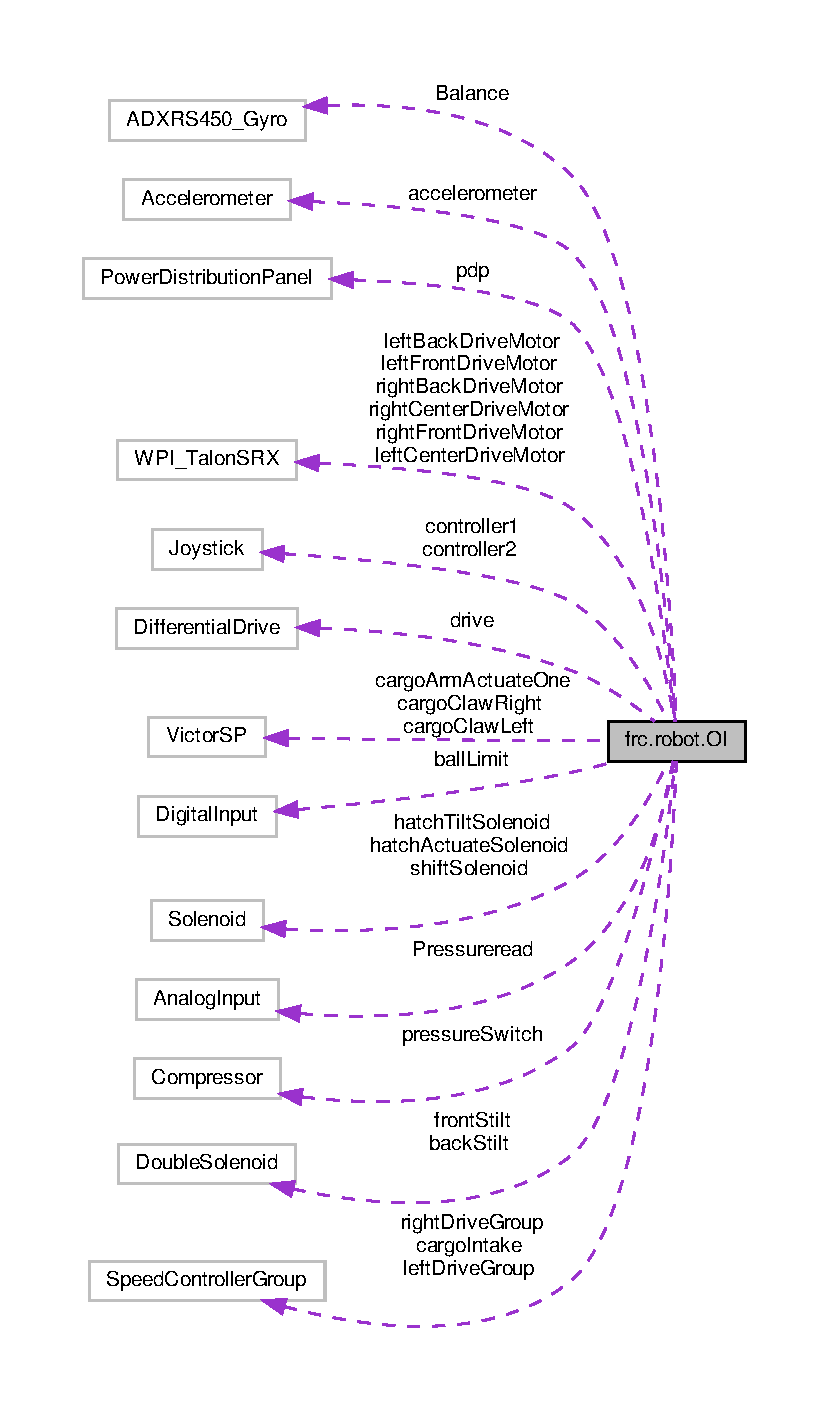
\includegraphics[height=550pt]{classfrc_1_1robot_1_1OI__coll__graph}
\end{center}
\end{figure}
\subsection*{Static Public Attributes}
\begin{DoxyCompactItemize}
\item 
static Power\+Distribution\+Panel \hyperlink{classfrc_1_1robot_1_1OI_a98d90326dfdaf14238d2f81c20c55f3f}{pdp} = new Power\+Distribution\+Panel(\hyperlink{classfrc_1_1robot_1_1RobotMap_af7db1426412719318df15f9838b70198}{Robot\+Map.\+pdp\+C\+AN})
\item 
static Joystick \hyperlink{classfrc_1_1robot_1_1OI_a06db411c1eebb80d10f685c57954bac9}{controller1} = new Joystick(\hyperlink{classfrc_1_1robot_1_1RobotMap_adf0118e5a9de03d6f71ea1e5a6a81cc9}{Robot\+Map.\+controller\+One\+Port})
\item 
static Joystick \hyperlink{classfrc_1_1robot_1_1OI_a749a3f830f90057dc4fd65e7f34a3251}{controller2} = new Joystick(\hyperlink{classfrc_1_1robot_1_1RobotMap_a762ebcaa07378c37d88654506850e07f}{Robot\+Map.\+controller\+Two\+Port})
\item 
static W\+P\+I\+\_\+\+Talon\+S\+RX \hyperlink{classfrc_1_1robot_1_1OI_a3f39e281419ebd60b94126e87e3ec81d}{left\+Front\+Drive\+Motor} = new W\+P\+I\+\_\+\+Talon\+S\+RX(\hyperlink{classfrc_1_1robot_1_1RobotMap_a2e3dbfb148d6fa2b7f430614887217f0}{Robot\+Map.\+left\+Front\+Drive\+C\+AN})
\item 
static W\+P\+I\+\_\+\+Talon\+S\+RX \hyperlink{classfrc_1_1robot_1_1OI_a8c33a9f0b9e366e48abd23ab01907e18}{left\+Center\+Drive\+Motor} = new W\+P\+I\+\_\+\+Talon\+S\+RX(\hyperlink{classfrc_1_1robot_1_1RobotMap_a9d04abf669a5ad42cb023e3ff3b56bcd}{Robot\+Map.\+left\+Center\+Drive\+C\+AN})
\item 
static W\+P\+I\+\_\+\+Talon\+S\+RX \hyperlink{classfrc_1_1robot_1_1OI_a88080d092baf8ece2c22f2ceec4f6f8f}{left\+Back\+Drive\+Motor} = new W\+P\+I\+\_\+\+Talon\+S\+RX(\hyperlink{classfrc_1_1robot_1_1RobotMap_a0f78f6850b0e060cc6acd88cc80ffa04}{Robot\+Map.\+left\+Back\+Drive\+C\+AN})
\item 
static W\+P\+I\+\_\+\+Talon\+S\+RX \hyperlink{classfrc_1_1robot_1_1OI_ae055ab4ea5a306737c950b1bfddf7352}{right\+Front\+Drive\+Motor} = new W\+P\+I\+\_\+\+Talon\+S\+RX(\hyperlink{classfrc_1_1robot_1_1RobotMap_a4ca461a7ad91df180971974fd6abc236}{Robot\+Map.\+right\+Front\+Drive\+C\+AN})
\item 
static W\+P\+I\+\_\+\+Talon\+S\+RX \hyperlink{classfrc_1_1robot_1_1OI_a9be3279c18d1f3433d6b07c706eb1457}{right\+Center\+Drive\+Motor} = new W\+P\+I\+\_\+\+Talon\+S\+RX(\hyperlink{classfrc_1_1robot_1_1RobotMap_a3ca36356410531e52126d2979ee17f13}{Robot\+Map.\+right\+Center\+Drive\+C\+AN})
\item 
static W\+P\+I\+\_\+\+Talon\+S\+RX \hyperlink{classfrc_1_1robot_1_1OI_a5f2937beffdc7dd1d937aaff36f20c1e}{right\+Back\+Drive\+Motor} = new W\+P\+I\+\_\+\+Talon\+S\+RX(\hyperlink{classfrc_1_1robot_1_1RobotMap_a0fb2fff6bf26e3f196d1cb02a89072c3}{Robot\+Map.\+right\+Back\+Drive\+C\+AN})
\item 
static Double\+Solenoid \hyperlink{classfrc_1_1robot_1_1OI_a4f6b2dd823bad92cfaf2e9ecc7c0b1ca}{front\+Stilt} = new Double\+Solenoid(14, 2, 3)
\item 
static Double\+Solenoid \hyperlink{classfrc_1_1robot_1_1OI_a89667abb08d7721a47088f0218fd5afa}{back\+Stilt} = new Double\+Solenoid(14, 6, 7)
\item 
static Speed\+Controller\+Group \hyperlink{classfrc_1_1robot_1_1OI_a6d76241e542ab271366e4cb4bf7b5133}{left\+Drive\+Group} = new Speed\+Controller\+Group(\hyperlink{classfrc_1_1robot_1_1OI_a8c33a9f0b9e366e48abd23ab01907e18}{left\+Center\+Drive\+Motor}, \hyperlink{classfrc_1_1robot_1_1OI_a88080d092baf8ece2c22f2ceec4f6f8f}{left\+Back\+Drive\+Motor},\hyperlink{classfrc_1_1robot_1_1OI_a3f39e281419ebd60b94126e87e3ec81d}{left\+Front\+Drive\+Motor})
\item 
static Speed\+Controller\+Group \hyperlink{classfrc_1_1robot_1_1OI_a1595c2b8ebd7e4e467027b2eb21983ee}{right\+Drive\+Group} = new Speed\+Controller\+Group(\hyperlink{classfrc_1_1robot_1_1OI_a9be3279c18d1f3433d6b07c706eb1457}{right\+Center\+Drive\+Motor}, \hyperlink{classfrc_1_1robot_1_1OI_a5f2937beffdc7dd1d937aaff36f20c1e}{right\+Back\+Drive\+Motor})
\item 
static Differential\+Drive \hyperlink{classfrc_1_1robot_1_1OI_a8527ec31aa37a3ff523e5ba857aba46f}{drive} = new Differential\+Drive(\hyperlink{classfrc_1_1robot_1_1OI_a6d76241e542ab271366e4cb4bf7b5133}{left\+Drive\+Group}, \hyperlink{classfrc_1_1robot_1_1OI_a1595c2b8ebd7e4e467027b2eb21983ee}{right\+Drive\+Group})
\item 
static Solenoid \hyperlink{classfrc_1_1robot_1_1OI_a63a56e8585378f6afe6f45facc98f494}{shift\+Solenoid} = new Solenoid(\hyperlink{classfrc_1_1robot_1_1RobotMap_a79a848df56d706c787d9a4f9a0434e7f}{Robot\+Map.\+P\+C\+M\+One\+C\+AN}, Robot\+Map.\+shift\+Solenoid)
\item 
static Solenoid \hyperlink{classfrc_1_1robot_1_1OI_a232ad4f80d75cd3d48c2067251c59817}{hatch\+Actuate\+Solenoid} = new Solenoid(\hyperlink{classfrc_1_1robot_1_1RobotMap_a79a848df56d706c787d9a4f9a0434e7f}{Robot\+Map.\+P\+C\+M\+One\+C\+AN}, \hyperlink{classfrc_1_1robot_1_1RobotMap_a7bec1963c7590911eb30697b0707d9b4}{Robot\+Map.\+hatch\+Actuate})
\item 
static Solenoid \hyperlink{classfrc_1_1robot_1_1OI_aa8cdb6b236dfb9fead12621b4f42c274}{hatch\+Tilt\+Solenoid} = new Solenoid(\hyperlink{classfrc_1_1robot_1_1RobotMap_a79a848df56d706c787d9a4f9a0434e7f}{Robot\+Map.\+P\+C\+M\+One\+C\+AN}, \hyperlink{classfrc_1_1robot_1_1RobotMap_a0c656cb43ea0fd37d6b94991e8473bf9}{Robot\+Map.\+hatch\+Tilt})
\item 
static Victor\+SP \hyperlink{classfrc_1_1robot_1_1OI_aeee9fe6efef4ea8f2558ccd2de43e71a}{cargo\+Arm\+Actuate\+One} = new Victor\+SP(\hyperlink{classfrc_1_1robot_1_1RobotMap_aaff9d0adef8e1f97db2ac47f985f044a}{Robot\+Map.\+cargo\+Arm\+Actuate\+One\+P\+WM})
\item 
static Victor\+SP \hyperlink{classfrc_1_1robot_1_1OI_a7ec725773fd1bb5dc4263980a232e75f}{cargo\+Claw\+Left} = new Victor\+SP(\hyperlink{classfrc_1_1robot_1_1RobotMap_aa5824f279bf68bbd68ae1ea3087c4b67}{Robot\+Map.\+cargo\+Claw\+Left\+Rotate\+P\+WM})
\item 
static Victor\+SP \hyperlink{classfrc_1_1robot_1_1OI_a32fd81c9a712924aa42a9eb74f278df1}{cargo\+Claw\+Right} = new Victor\+SP(\hyperlink{classfrc_1_1robot_1_1RobotMap_a108c3b97c541e7ed5a152cea66981231}{Robot\+Map.\+cargo\+Claw\+Right\+Rotate\+P\+WM})
\item 
static Speed\+Controller\+Group \hyperlink{classfrc_1_1robot_1_1OI_a40d2adcc988805032885ba668fc6f86f}{cargo\+Intake} = new Speed\+Controller\+Group(\hyperlink{classfrc_1_1robot_1_1OI_a7ec725773fd1bb5dc4263980a232e75f}{cargo\+Claw\+Left}, \hyperlink{classfrc_1_1robot_1_1OI_a32fd81c9a712924aa42a9eb74f278df1}{cargo\+Claw\+Right})
\item 
static Digital\+Input \hyperlink{classfrc_1_1robot_1_1OI_aebf7c01734a48f269b40f7b1f1125f10}{ball\+Limit} = new Digital\+Input(\hyperlink{classfrc_1_1robot_1_1RobotMap_a83f3eec03443af1dbe44492871796c92}{Robot\+Map.\+ball\+Limit\+D\+IO})
\item 
static Accelerometer \hyperlink{classfrc_1_1robot_1_1OI_a57e609e018f3013d5beb8bffa5771df0}{accelerometer} = new Built\+In\+Accelerometer(Accelerometer.\+Range.\+k4G)
\item 
static Compressor \hyperlink{classfrc_1_1robot_1_1OI_a68157a4a30cc0fae8bc36ae0ac999c82}{pressure\+Switch} = new Compressor()
\item 
static Analog\+Input \hyperlink{classfrc_1_1robot_1_1OI_a763d5acad9b29d4b29b0fff838059571}{Pressureread} = new Analog\+Input(\hyperlink{classfrc_1_1robot_1_1RobotMap_a10cc39db919c29133e2bc774281804b0}{Robot\+Map.\+Pressure\+\_\+read})
\item 
static A\+D\+X\+R\+S450\+\_\+\+Gyro \hyperlink{classfrc_1_1robot_1_1OI_a951d7ff102fca8319e5a9401a0f2214b}{Balance} = new A\+D\+X\+R\+S450\+\_\+\+Gyro()
\end{DoxyCompactItemize}


\subsection{Detailed Description}
This class is the glue that binds the controls on the physical operator interface to the commands and command groups that allow control of the robot. 

Definition at line 30 of file O\+I.\+java.



\subsection{Member Data Documentation}
\mbox{\Hypertarget{classfrc_1_1robot_1_1OI_a57e609e018f3013d5beb8bffa5771df0}\label{classfrc_1_1robot_1_1OI_a57e609e018f3013d5beb8bffa5771df0}} 
\index{frc\+::robot\+::\+OI@{frc\+::robot\+::\+OI}!accelerometer@{accelerometer}}
\index{accelerometer@{accelerometer}!frc\+::robot\+::\+OI@{frc\+::robot\+::\+OI}}
\subsubsection{\texorpdfstring{accelerometer}{accelerometer}}
{\footnotesize\ttfamily Accelerometer frc.\+robot.\+O\+I.\+accelerometer = new Built\+In\+Accelerometer(Accelerometer.\+Range.\+k4G)\hspace{0.3cm}{\ttfamily [static]}}



Definition at line 61 of file O\+I.\+java.

\mbox{\Hypertarget{classfrc_1_1robot_1_1OI_a89667abb08d7721a47088f0218fd5afa}\label{classfrc_1_1robot_1_1OI_a89667abb08d7721a47088f0218fd5afa}} 
\index{frc\+::robot\+::\+OI@{frc\+::robot\+::\+OI}!back\+Stilt@{back\+Stilt}}
\index{back\+Stilt@{back\+Stilt}!frc\+::robot\+::\+OI@{frc\+::robot\+::\+OI}}
\subsubsection{\texorpdfstring{back\+Stilt}{backStilt}}
{\footnotesize\ttfamily Double\+Solenoid frc.\+robot.\+O\+I.\+back\+Stilt = new Double\+Solenoid(14, 6, 7)\hspace{0.3cm}{\ttfamily [static]}}



Definition at line 44 of file O\+I.\+java.

\mbox{\Hypertarget{classfrc_1_1robot_1_1OI_a951d7ff102fca8319e5a9401a0f2214b}\label{classfrc_1_1robot_1_1OI_a951d7ff102fca8319e5a9401a0f2214b}} 
\index{frc\+::robot\+::\+OI@{frc\+::robot\+::\+OI}!Balance@{Balance}}
\index{Balance@{Balance}!frc\+::robot\+::\+OI@{frc\+::robot\+::\+OI}}
\subsubsection{\texorpdfstring{Balance}{Balance}}
{\footnotesize\ttfamily A\+D\+X\+R\+S450\+\_\+\+Gyro frc.\+robot.\+O\+I.\+Balance = new A\+D\+X\+R\+S450\+\_\+\+Gyro()\hspace{0.3cm}{\ttfamily [static]}}



Definition at line 65 of file O\+I.\+java.

\mbox{\Hypertarget{classfrc_1_1robot_1_1OI_aebf7c01734a48f269b40f7b1f1125f10}\label{classfrc_1_1robot_1_1OI_aebf7c01734a48f269b40f7b1f1125f10}} 
\index{frc\+::robot\+::\+OI@{frc\+::robot\+::\+OI}!ball\+Limit@{ball\+Limit}}
\index{ball\+Limit@{ball\+Limit}!frc\+::robot\+::\+OI@{frc\+::robot\+::\+OI}}
\subsubsection{\texorpdfstring{ball\+Limit}{ballLimit}}
{\footnotesize\ttfamily Digital\+Input frc.\+robot.\+O\+I.\+ball\+Limit = new Digital\+Input(\hyperlink{classfrc_1_1robot_1_1RobotMap_a83f3eec03443af1dbe44492871796c92}{Robot\+Map.\+ball\+Limit\+D\+IO})\hspace{0.3cm}{\ttfamily [static]}}



Definition at line 60 of file O\+I.\+java.

\mbox{\Hypertarget{classfrc_1_1robot_1_1OI_aeee9fe6efef4ea8f2558ccd2de43e71a}\label{classfrc_1_1robot_1_1OI_aeee9fe6efef4ea8f2558ccd2de43e71a}} 
\index{frc\+::robot\+::\+OI@{frc\+::robot\+::\+OI}!cargo\+Arm\+Actuate\+One@{cargo\+Arm\+Actuate\+One}}
\index{cargo\+Arm\+Actuate\+One@{cargo\+Arm\+Actuate\+One}!frc\+::robot\+::\+OI@{frc\+::robot\+::\+OI}}
\subsubsection{\texorpdfstring{cargo\+Arm\+Actuate\+One}{cargoArmActuateOne}}
{\footnotesize\ttfamily Victor\+SP frc.\+robot.\+O\+I.\+cargo\+Arm\+Actuate\+One = new Victor\+SP(\hyperlink{classfrc_1_1robot_1_1RobotMap_aaff9d0adef8e1f97db2ac47f985f044a}{Robot\+Map.\+cargo\+Arm\+Actuate\+One\+P\+WM})\hspace{0.3cm}{\ttfamily [static]}}



Definition at line 55 of file O\+I.\+java.

\mbox{\Hypertarget{classfrc_1_1robot_1_1OI_a7ec725773fd1bb5dc4263980a232e75f}\label{classfrc_1_1robot_1_1OI_a7ec725773fd1bb5dc4263980a232e75f}} 
\index{frc\+::robot\+::\+OI@{frc\+::robot\+::\+OI}!cargo\+Claw\+Left@{cargo\+Claw\+Left}}
\index{cargo\+Claw\+Left@{cargo\+Claw\+Left}!frc\+::robot\+::\+OI@{frc\+::robot\+::\+OI}}
\subsubsection{\texorpdfstring{cargo\+Claw\+Left}{cargoClawLeft}}
{\footnotesize\ttfamily Victor\+SP frc.\+robot.\+O\+I.\+cargo\+Claw\+Left = new Victor\+SP(\hyperlink{classfrc_1_1robot_1_1RobotMap_aa5824f279bf68bbd68ae1ea3087c4b67}{Robot\+Map.\+cargo\+Claw\+Left\+Rotate\+P\+WM})\hspace{0.3cm}{\ttfamily [static]}}



Definition at line 56 of file O\+I.\+java.

\mbox{\Hypertarget{classfrc_1_1robot_1_1OI_a32fd81c9a712924aa42a9eb74f278df1}\label{classfrc_1_1robot_1_1OI_a32fd81c9a712924aa42a9eb74f278df1}} 
\index{frc\+::robot\+::\+OI@{frc\+::robot\+::\+OI}!cargo\+Claw\+Right@{cargo\+Claw\+Right}}
\index{cargo\+Claw\+Right@{cargo\+Claw\+Right}!frc\+::robot\+::\+OI@{frc\+::robot\+::\+OI}}
\subsubsection{\texorpdfstring{cargo\+Claw\+Right}{cargoClawRight}}
{\footnotesize\ttfamily Victor\+SP frc.\+robot.\+O\+I.\+cargo\+Claw\+Right = new Victor\+SP(\hyperlink{classfrc_1_1robot_1_1RobotMap_a108c3b97c541e7ed5a152cea66981231}{Robot\+Map.\+cargo\+Claw\+Right\+Rotate\+P\+WM})\hspace{0.3cm}{\ttfamily [static]}}



Definition at line 57 of file O\+I.\+java.

\mbox{\Hypertarget{classfrc_1_1robot_1_1OI_a40d2adcc988805032885ba668fc6f86f}\label{classfrc_1_1robot_1_1OI_a40d2adcc988805032885ba668fc6f86f}} 
\index{frc\+::robot\+::\+OI@{frc\+::robot\+::\+OI}!cargo\+Intake@{cargo\+Intake}}
\index{cargo\+Intake@{cargo\+Intake}!frc\+::robot\+::\+OI@{frc\+::robot\+::\+OI}}
\subsubsection{\texorpdfstring{cargo\+Intake}{cargoIntake}}
{\footnotesize\ttfamily Speed\+Controller\+Group frc.\+robot.\+O\+I.\+cargo\+Intake = new Speed\+Controller\+Group(\hyperlink{classfrc_1_1robot_1_1OI_a7ec725773fd1bb5dc4263980a232e75f}{cargo\+Claw\+Left}, \hyperlink{classfrc_1_1robot_1_1OI_a32fd81c9a712924aa42a9eb74f278df1}{cargo\+Claw\+Right})\hspace{0.3cm}{\ttfamily [static]}}



Definition at line 58 of file O\+I.\+java.

\mbox{\Hypertarget{classfrc_1_1robot_1_1OI_a06db411c1eebb80d10f685c57954bac9}\label{classfrc_1_1robot_1_1OI_a06db411c1eebb80d10f685c57954bac9}} 
\index{frc\+::robot\+::\+OI@{frc\+::robot\+::\+OI}!controller1@{controller1}}
\index{controller1@{controller1}!frc\+::robot\+::\+OI@{frc\+::robot\+::\+OI}}
\subsubsection{\texorpdfstring{controller1}{controller1}}
{\footnotesize\ttfamily Joystick frc.\+robot.\+O\+I.\+controller1 = new Joystick(\hyperlink{classfrc_1_1robot_1_1RobotMap_adf0118e5a9de03d6f71ea1e5a6a81cc9}{Robot\+Map.\+controller\+One\+Port})\hspace{0.3cm}{\ttfamily [static]}}



Definition at line 33 of file O\+I.\+java.

\mbox{\Hypertarget{classfrc_1_1robot_1_1OI_a749a3f830f90057dc4fd65e7f34a3251}\label{classfrc_1_1robot_1_1OI_a749a3f830f90057dc4fd65e7f34a3251}} 
\index{frc\+::robot\+::\+OI@{frc\+::robot\+::\+OI}!controller2@{controller2}}
\index{controller2@{controller2}!frc\+::robot\+::\+OI@{frc\+::robot\+::\+OI}}
\subsubsection{\texorpdfstring{controller2}{controller2}}
{\footnotesize\ttfamily Joystick frc.\+robot.\+O\+I.\+controller2 = new Joystick(\hyperlink{classfrc_1_1robot_1_1RobotMap_a762ebcaa07378c37d88654506850e07f}{Robot\+Map.\+controller\+Two\+Port})\hspace{0.3cm}{\ttfamily [static]}}



Definition at line 34 of file O\+I.\+java.

\mbox{\Hypertarget{classfrc_1_1robot_1_1OI_a8527ec31aa37a3ff523e5ba857aba46f}\label{classfrc_1_1robot_1_1OI_a8527ec31aa37a3ff523e5ba857aba46f}} 
\index{frc\+::robot\+::\+OI@{frc\+::robot\+::\+OI}!drive@{drive}}
\index{drive@{drive}!frc\+::robot\+::\+OI@{frc\+::robot\+::\+OI}}
\subsubsection{\texorpdfstring{drive}{drive}}
{\footnotesize\ttfamily Differential\+Drive frc.\+robot.\+O\+I.\+drive = new Differential\+Drive(\hyperlink{classfrc_1_1robot_1_1OI_a6d76241e542ab271366e4cb4bf7b5133}{left\+Drive\+Group}, \hyperlink{classfrc_1_1robot_1_1OI_a1595c2b8ebd7e4e467027b2eb21983ee}{right\+Drive\+Group})\hspace{0.3cm}{\ttfamily [static]}}



Definition at line 49 of file O\+I.\+java.

\mbox{\Hypertarget{classfrc_1_1robot_1_1OI_a4f6b2dd823bad92cfaf2e9ecc7c0b1ca}\label{classfrc_1_1robot_1_1OI_a4f6b2dd823bad92cfaf2e9ecc7c0b1ca}} 
\index{frc\+::robot\+::\+OI@{frc\+::robot\+::\+OI}!front\+Stilt@{front\+Stilt}}
\index{front\+Stilt@{front\+Stilt}!frc\+::robot\+::\+OI@{frc\+::robot\+::\+OI}}
\subsubsection{\texorpdfstring{front\+Stilt}{frontStilt}}
{\footnotesize\ttfamily Double\+Solenoid frc.\+robot.\+O\+I.\+front\+Stilt = new Double\+Solenoid(14, 2, 3)\hspace{0.3cm}{\ttfamily [static]}}



Definition at line 43 of file O\+I.\+java.

\mbox{\Hypertarget{classfrc_1_1robot_1_1OI_a232ad4f80d75cd3d48c2067251c59817}\label{classfrc_1_1robot_1_1OI_a232ad4f80d75cd3d48c2067251c59817}} 
\index{frc\+::robot\+::\+OI@{frc\+::robot\+::\+OI}!hatch\+Actuate\+Solenoid@{hatch\+Actuate\+Solenoid}}
\index{hatch\+Actuate\+Solenoid@{hatch\+Actuate\+Solenoid}!frc\+::robot\+::\+OI@{frc\+::robot\+::\+OI}}
\subsubsection{\texorpdfstring{hatch\+Actuate\+Solenoid}{hatchActuateSolenoid}}
{\footnotesize\ttfamily Solenoid frc.\+robot.\+O\+I.\+hatch\+Actuate\+Solenoid = new Solenoid(\hyperlink{classfrc_1_1robot_1_1RobotMap_a79a848df56d706c787d9a4f9a0434e7f}{Robot\+Map.\+P\+C\+M\+One\+C\+AN}, \hyperlink{classfrc_1_1robot_1_1RobotMap_a7bec1963c7590911eb30697b0707d9b4}{Robot\+Map.\+hatch\+Actuate})\hspace{0.3cm}{\ttfamily [static]}}



Definition at line 52 of file O\+I.\+java.

\mbox{\Hypertarget{classfrc_1_1robot_1_1OI_aa8cdb6b236dfb9fead12621b4f42c274}\label{classfrc_1_1robot_1_1OI_aa8cdb6b236dfb9fead12621b4f42c274}} 
\index{frc\+::robot\+::\+OI@{frc\+::robot\+::\+OI}!hatch\+Tilt\+Solenoid@{hatch\+Tilt\+Solenoid}}
\index{hatch\+Tilt\+Solenoid@{hatch\+Tilt\+Solenoid}!frc\+::robot\+::\+OI@{frc\+::robot\+::\+OI}}
\subsubsection{\texorpdfstring{hatch\+Tilt\+Solenoid}{hatchTiltSolenoid}}
{\footnotesize\ttfamily Solenoid frc.\+robot.\+O\+I.\+hatch\+Tilt\+Solenoid = new Solenoid(\hyperlink{classfrc_1_1robot_1_1RobotMap_a79a848df56d706c787d9a4f9a0434e7f}{Robot\+Map.\+P\+C\+M\+One\+C\+AN}, \hyperlink{classfrc_1_1robot_1_1RobotMap_a0c656cb43ea0fd37d6b94991e8473bf9}{Robot\+Map.\+hatch\+Tilt})\hspace{0.3cm}{\ttfamily [static]}}



Definition at line 53 of file O\+I.\+java.

\mbox{\Hypertarget{classfrc_1_1robot_1_1OI_a88080d092baf8ece2c22f2ceec4f6f8f}\label{classfrc_1_1robot_1_1OI_a88080d092baf8ece2c22f2ceec4f6f8f}} 
\index{frc\+::robot\+::\+OI@{frc\+::robot\+::\+OI}!left\+Back\+Drive\+Motor@{left\+Back\+Drive\+Motor}}
\index{left\+Back\+Drive\+Motor@{left\+Back\+Drive\+Motor}!frc\+::robot\+::\+OI@{frc\+::robot\+::\+OI}}
\subsubsection{\texorpdfstring{left\+Back\+Drive\+Motor}{leftBackDriveMotor}}
{\footnotesize\ttfamily W\+P\+I\+\_\+\+Talon\+S\+RX frc.\+robot.\+O\+I.\+left\+Back\+Drive\+Motor = new W\+P\+I\+\_\+\+Talon\+S\+RX(\hyperlink{classfrc_1_1robot_1_1RobotMap_a0f78f6850b0e060cc6acd88cc80ffa04}{Robot\+Map.\+left\+Back\+Drive\+C\+AN})\hspace{0.3cm}{\ttfamily [static]}}



Definition at line 38 of file O\+I.\+java.

\mbox{\Hypertarget{classfrc_1_1robot_1_1OI_a8c33a9f0b9e366e48abd23ab01907e18}\label{classfrc_1_1robot_1_1OI_a8c33a9f0b9e366e48abd23ab01907e18}} 
\index{frc\+::robot\+::\+OI@{frc\+::robot\+::\+OI}!left\+Center\+Drive\+Motor@{left\+Center\+Drive\+Motor}}
\index{left\+Center\+Drive\+Motor@{left\+Center\+Drive\+Motor}!frc\+::robot\+::\+OI@{frc\+::robot\+::\+OI}}
\subsubsection{\texorpdfstring{left\+Center\+Drive\+Motor}{leftCenterDriveMotor}}
{\footnotesize\ttfamily W\+P\+I\+\_\+\+Talon\+S\+RX frc.\+robot.\+O\+I.\+left\+Center\+Drive\+Motor = new W\+P\+I\+\_\+\+Talon\+S\+RX(\hyperlink{classfrc_1_1robot_1_1RobotMap_a9d04abf669a5ad42cb023e3ff3b56bcd}{Robot\+Map.\+left\+Center\+Drive\+C\+AN})\hspace{0.3cm}{\ttfamily [static]}}



Definition at line 37 of file O\+I.\+java.

\mbox{\Hypertarget{classfrc_1_1robot_1_1OI_a6d76241e542ab271366e4cb4bf7b5133}\label{classfrc_1_1robot_1_1OI_a6d76241e542ab271366e4cb4bf7b5133}} 
\index{frc\+::robot\+::\+OI@{frc\+::robot\+::\+OI}!left\+Drive\+Group@{left\+Drive\+Group}}
\index{left\+Drive\+Group@{left\+Drive\+Group}!frc\+::robot\+::\+OI@{frc\+::robot\+::\+OI}}
\subsubsection{\texorpdfstring{left\+Drive\+Group}{leftDriveGroup}}
{\footnotesize\ttfamily Speed\+Controller\+Group frc.\+robot.\+O\+I.\+left\+Drive\+Group = new Speed\+Controller\+Group(\hyperlink{classfrc_1_1robot_1_1OI_a8c33a9f0b9e366e48abd23ab01907e18}{left\+Center\+Drive\+Motor}, \hyperlink{classfrc_1_1robot_1_1OI_a88080d092baf8ece2c22f2ceec4f6f8f}{left\+Back\+Drive\+Motor},\hyperlink{classfrc_1_1robot_1_1OI_a3f39e281419ebd60b94126e87e3ec81d}{left\+Front\+Drive\+Motor})\hspace{0.3cm}{\ttfamily [static]}}



Definition at line 46 of file O\+I.\+java.

\mbox{\Hypertarget{classfrc_1_1robot_1_1OI_a3f39e281419ebd60b94126e87e3ec81d}\label{classfrc_1_1robot_1_1OI_a3f39e281419ebd60b94126e87e3ec81d}} 
\index{frc\+::robot\+::\+OI@{frc\+::robot\+::\+OI}!left\+Front\+Drive\+Motor@{left\+Front\+Drive\+Motor}}
\index{left\+Front\+Drive\+Motor@{left\+Front\+Drive\+Motor}!frc\+::robot\+::\+OI@{frc\+::robot\+::\+OI}}
\subsubsection{\texorpdfstring{left\+Front\+Drive\+Motor}{leftFrontDriveMotor}}
{\footnotesize\ttfamily W\+P\+I\+\_\+\+Talon\+S\+RX frc.\+robot.\+O\+I.\+left\+Front\+Drive\+Motor = new W\+P\+I\+\_\+\+Talon\+S\+RX(\hyperlink{classfrc_1_1robot_1_1RobotMap_a2e3dbfb148d6fa2b7f430614887217f0}{Robot\+Map.\+left\+Front\+Drive\+C\+AN})\hspace{0.3cm}{\ttfamily [static]}}



Definition at line 36 of file O\+I.\+java.

\mbox{\Hypertarget{classfrc_1_1robot_1_1OI_a98d90326dfdaf14238d2f81c20c55f3f}\label{classfrc_1_1robot_1_1OI_a98d90326dfdaf14238d2f81c20c55f3f}} 
\index{frc\+::robot\+::\+OI@{frc\+::robot\+::\+OI}!pdp@{pdp}}
\index{pdp@{pdp}!frc\+::robot\+::\+OI@{frc\+::robot\+::\+OI}}
\subsubsection{\texorpdfstring{pdp}{pdp}}
{\footnotesize\ttfamily Power\+Distribution\+Panel frc.\+robot.\+O\+I.\+pdp = new Power\+Distribution\+Panel(\hyperlink{classfrc_1_1robot_1_1RobotMap_af7db1426412719318df15f9838b70198}{Robot\+Map.\+pdp\+C\+AN})\hspace{0.3cm}{\ttfamily [static]}}



Definition at line 31 of file O\+I.\+java.

\mbox{\Hypertarget{classfrc_1_1robot_1_1OI_a763d5acad9b29d4b29b0fff838059571}\label{classfrc_1_1robot_1_1OI_a763d5acad9b29d4b29b0fff838059571}} 
\index{frc\+::robot\+::\+OI@{frc\+::robot\+::\+OI}!Pressureread@{Pressureread}}
\index{Pressureread@{Pressureread}!frc\+::robot\+::\+OI@{frc\+::robot\+::\+OI}}
\subsubsection{\texorpdfstring{Pressureread}{Pressureread}}
{\footnotesize\ttfamily Analog\+Input frc.\+robot.\+O\+I.\+Pressureread = new Analog\+Input(\hyperlink{classfrc_1_1robot_1_1RobotMap_a10cc39db919c29133e2bc774281804b0}{Robot\+Map.\+Pressure\+\_\+read})\hspace{0.3cm}{\ttfamily [static]}}



Definition at line 64 of file O\+I.\+java.

\mbox{\Hypertarget{classfrc_1_1robot_1_1OI_a68157a4a30cc0fae8bc36ae0ac999c82}\label{classfrc_1_1robot_1_1OI_a68157a4a30cc0fae8bc36ae0ac999c82}} 
\index{frc\+::robot\+::\+OI@{frc\+::robot\+::\+OI}!pressure\+Switch@{pressure\+Switch}}
\index{pressure\+Switch@{pressure\+Switch}!frc\+::robot\+::\+OI@{frc\+::robot\+::\+OI}}
\subsubsection{\texorpdfstring{pressure\+Switch}{pressureSwitch}}
{\footnotesize\ttfamily Compressor frc.\+robot.\+O\+I.\+pressure\+Switch = new Compressor()\hspace{0.3cm}{\ttfamily [static]}}



Definition at line 62 of file O\+I.\+java.

\mbox{\Hypertarget{classfrc_1_1robot_1_1OI_a5f2937beffdc7dd1d937aaff36f20c1e}\label{classfrc_1_1robot_1_1OI_a5f2937beffdc7dd1d937aaff36f20c1e}} 
\index{frc\+::robot\+::\+OI@{frc\+::robot\+::\+OI}!right\+Back\+Drive\+Motor@{right\+Back\+Drive\+Motor}}
\index{right\+Back\+Drive\+Motor@{right\+Back\+Drive\+Motor}!frc\+::robot\+::\+OI@{frc\+::robot\+::\+OI}}
\subsubsection{\texorpdfstring{right\+Back\+Drive\+Motor}{rightBackDriveMotor}}
{\footnotesize\ttfamily W\+P\+I\+\_\+\+Talon\+S\+RX frc.\+robot.\+O\+I.\+right\+Back\+Drive\+Motor = new W\+P\+I\+\_\+\+Talon\+S\+RX(\hyperlink{classfrc_1_1robot_1_1RobotMap_a0fb2fff6bf26e3f196d1cb02a89072c3}{Robot\+Map.\+right\+Back\+Drive\+C\+AN})\hspace{0.3cm}{\ttfamily [static]}}



Definition at line 41 of file O\+I.\+java.

\mbox{\Hypertarget{classfrc_1_1robot_1_1OI_a9be3279c18d1f3433d6b07c706eb1457}\label{classfrc_1_1robot_1_1OI_a9be3279c18d1f3433d6b07c706eb1457}} 
\index{frc\+::robot\+::\+OI@{frc\+::robot\+::\+OI}!right\+Center\+Drive\+Motor@{right\+Center\+Drive\+Motor}}
\index{right\+Center\+Drive\+Motor@{right\+Center\+Drive\+Motor}!frc\+::robot\+::\+OI@{frc\+::robot\+::\+OI}}
\subsubsection{\texorpdfstring{right\+Center\+Drive\+Motor}{rightCenterDriveMotor}}
{\footnotesize\ttfamily W\+P\+I\+\_\+\+Talon\+S\+RX frc.\+robot.\+O\+I.\+right\+Center\+Drive\+Motor = new W\+P\+I\+\_\+\+Talon\+S\+RX(\hyperlink{classfrc_1_1robot_1_1RobotMap_a3ca36356410531e52126d2979ee17f13}{Robot\+Map.\+right\+Center\+Drive\+C\+AN})\hspace{0.3cm}{\ttfamily [static]}}



Definition at line 40 of file O\+I.\+java.

\mbox{\Hypertarget{classfrc_1_1robot_1_1OI_a1595c2b8ebd7e4e467027b2eb21983ee}\label{classfrc_1_1robot_1_1OI_a1595c2b8ebd7e4e467027b2eb21983ee}} 
\index{frc\+::robot\+::\+OI@{frc\+::robot\+::\+OI}!right\+Drive\+Group@{right\+Drive\+Group}}
\index{right\+Drive\+Group@{right\+Drive\+Group}!frc\+::robot\+::\+OI@{frc\+::robot\+::\+OI}}
\subsubsection{\texorpdfstring{right\+Drive\+Group}{rightDriveGroup}}
{\footnotesize\ttfamily Speed\+Controller\+Group frc.\+robot.\+O\+I.\+right\+Drive\+Group = new Speed\+Controller\+Group(\hyperlink{classfrc_1_1robot_1_1OI_a9be3279c18d1f3433d6b07c706eb1457}{right\+Center\+Drive\+Motor}, \hyperlink{classfrc_1_1robot_1_1OI_a5f2937beffdc7dd1d937aaff36f20c1e}{right\+Back\+Drive\+Motor})\hspace{0.3cm}{\ttfamily [static]}}



Definition at line 47 of file O\+I.\+java.

\mbox{\Hypertarget{classfrc_1_1robot_1_1OI_ae055ab4ea5a306737c950b1bfddf7352}\label{classfrc_1_1robot_1_1OI_ae055ab4ea5a306737c950b1bfddf7352}} 
\index{frc\+::robot\+::\+OI@{frc\+::robot\+::\+OI}!right\+Front\+Drive\+Motor@{right\+Front\+Drive\+Motor}}
\index{right\+Front\+Drive\+Motor@{right\+Front\+Drive\+Motor}!frc\+::robot\+::\+OI@{frc\+::robot\+::\+OI}}
\subsubsection{\texorpdfstring{right\+Front\+Drive\+Motor}{rightFrontDriveMotor}}
{\footnotesize\ttfamily W\+P\+I\+\_\+\+Talon\+S\+RX frc.\+robot.\+O\+I.\+right\+Front\+Drive\+Motor = new W\+P\+I\+\_\+\+Talon\+S\+RX(\hyperlink{classfrc_1_1robot_1_1RobotMap_a4ca461a7ad91df180971974fd6abc236}{Robot\+Map.\+right\+Front\+Drive\+C\+AN})\hspace{0.3cm}{\ttfamily [static]}}



Definition at line 39 of file O\+I.\+java.

\mbox{\Hypertarget{classfrc_1_1robot_1_1OI_a63a56e8585378f6afe6f45facc98f494}\label{classfrc_1_1robot_1_1OI_a63a56e8585378f6afe6f45facc98f494}} 
\index{frc\+::robot\+::\+OI@{frc\+::robot\+::\+OI}!shift\+Solenoid@{shift\+Solenoid}}
\index{shift\+Solenoid@{shift\+Solenoid}!frc\+::robot\+::\+OI@{frc\+::robot\+::\+OI}}
\subsubsection{\texorpdfstring{shift\+Solenoid}{shiftSolenoid}}
{\footnotesize\ttfamily Solenoid frc.\+robot.\+O\+I.\+shift\+Solenoid = new Solenoid(\hyperlink{classfrc_1_1robot_1_1RobotMap_a79a848df56d706c787d9a4f9a0434e7f}{Robot\+Map.\+P\+C\+M\+One\+C\+AN}, Robot\+Map.\+shift\+Solenoid)\hspace{0.3cm}{\ttfamily [static]}}



Definition at line 51 of file O\+I.\+java.



The documentation for this class was generated from the following file\+:\begin{DoxyCompactItemize}
\item 
src/main/java/frc/robot/\hyperlink{OI_8java}{O\+I.\+java}\end{DoxyCompactItemize}

\hypertarget{classfrc_1_1robot_1_1Robot}{}\section{frc.\+robot.\+Robot Class Reference}
\label{classfrc_1_1robot_1_1Robot}\index{frc.\+robot.\+Robot@{frc.\+robot.\+Robot}}


Inheritance diagram for frc.\+robot.\+Robot\+:\nopagebreak
\begin{figure}[H]
\begin{center}
\leavevmode
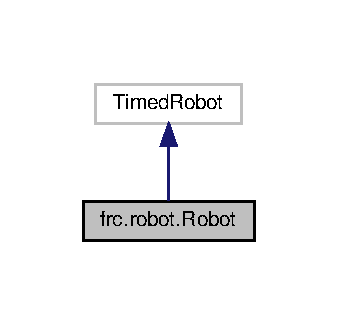
\includegraphics[width=162pt]{classfrc_1_1robot_1_1Robot__inherit__graph}
\end{center}
\end{figure}


Collaboration diagram for frc.\+robot.\+Robot\+:\nopagebreak
\begin{figure}[H]
\begin{center}
\leavevmode
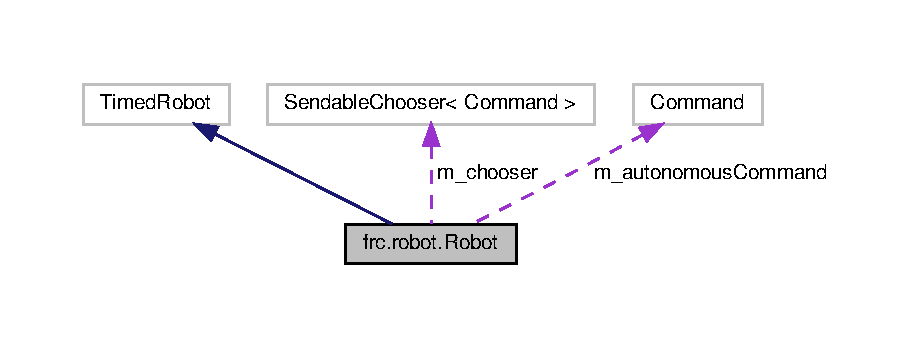
\includegraphics[width=350pt]{classfrc_1_1robot_1_1Robot__coll__graph}
\end{center}
\end{figure}
\subsection*{Public Member Functions}
\begin{DoxyCompactItemize}
\item 
void \hyperlink{classfrc_1_1robot_1_1Robot_a1d28582cf3dc31568c3581f631c92f13}{robot\+Init} ()
\item 
void \hyperlink{classfrc_1_1robot_1_1Robot_a7e63e32ebe8ad3d33bbc3b09092a9f1f}{robot\+Periodic} ()
\item 
void \hyperlink{classfrc_1_1robot_1_1Robot_ac19810fbf26efd4cd47cbd7568b4ad2a}{disabled\+Init} ()
\item 
void \hyperlink{classfrc_1_1robot_1_1Robot_a2bc1b0ce100e4783ba3d549e6ac07ae3}{disabled\+Periodic} ()
\item 
void \hyperlink{classfrc_1_1robot_1_1Robot_a5b1c022cd3e2b9f6e5dde62571839173}{autonomous\+Init} ()
\item 
void \hyperlink{classfrc_1_1robot_1_1Robot_a7dcfe7d0d65d1051eb095b8eb1aebd72}{autonomous\+Periodic} ()
\begin{DoxyCompactList}\small\item\em This function is called periodically during autonomous. \end{DoxyCompactList}\item 
void \hyperlink{classfrc_1_1robot_1_1Robot_a209dbf07bfec75d73fa53126a8e31b88}{teleop\+Init} ()
\item 
void \hyperlink{classfrc_1_1robot_1_1Robot_ae807171661cbc29081bc10f06d6831e7}{teleop\+Periodic} ()
\begin{DoxyCompactList}\small\item\em This function is called periodically during Teleop. \end{DoxyCompactList}\item 
void \hyperlink{classfrc_1_1robot_1_1Robot_abd152f34b9f33d5cdf835aa61331f33e}{test\+Periodic} ()
\end{DoxyCompactItemize}


\subsection{Detailed Description}


Definition at line 19 of file Robot.\+java.



\subsection{Member Function Documentation}
\mbox{\Hypertarget{classfrc_1_1robot_1_1Robot_a5b1c022cd3e2b9f6e5dde62571839173}\label{classfrc_1_1robot_1_1Robot_a5b1c022cd3e2b9f6e5dde62571839173}} 
\index{frc\+::robot\+::\+Robot@{frc\+::robot\+::\+Robot}!autonomous\+Init@{autonomous\+Init}}
\index{autonomous\+Init@{autonomous\+Init}!frc\+::robot\+::\+Robot@{frc\+::robot\+::\+Robot}}
\subsubsection{\texorpdfstring{autonomous\+Init()}{autonomousInit()}}
{\footnotesize\ttfamily void frc.\+robot.\+Robot.\+autonomous\+Init (\begin{DoxyParamCaption}{ }\end{DoxyParamCaption})}



Definition at line 44 of file Robot.\+java.

\mbox{\Hypertarget{classfrc_1_1robot_1_1Robot_a7dcfe7d0d65d1051eb095b8eb1aebd72}\label{classfrc_1_1robot_1_1Robot_a7dcfe7d0d65d1051eb095b8eb1aebd72}} 
\index{frc\+::robot\+::\+Robot@{frc\+::robot\+::\+Robot}!autonomous\+Periodic@{autonomous\+Periodic}}
\index{autonomous\+Periodic@{autonomous\+Periodic}!frc\+::robot\+::\+Robot@{frc\+::robot\+::\+Robot}}
\subsubsection{\texorpdfstring{autonomous\+Periodic()}{autonomousPeriodic()}}
{\footnotesize\ttfamily void frc.\+robot.\+Robot.\+autonomous\+Periodic (\begin{DoxyParamCaption}{ }\end{DoxyParamCaption})}



This function is called periodically during autonomous. 



Definition at line 52 of file Robot.\+java.

\mbox{\Hypertarget{classfrc_1_1robot_1_1Robot_ac19810fbf26efd4cd47cbd7568b4ad2a}\label{classfrc_1_1robot_1_1Robot_ac19810fbf26efd4cd47cbd7568b4ad2a}} 
\index{frc\+::robot\+::\+Robot@{frc\+::robot\+::\+Robot}!disabled\+Init@{disabled\+Init}}
\index{disabled\+Init@{disabled\+Init}!frc\+::robot\+::\+Robot@{frc\+::robot\+::\+Robot}}
\subsubsection{\texorpdfstring{disabled\+Init()}{disabledInit()}}
{\footnotesize\ttfamily void frc.\+robot.\+Robot.\+disabled\+Init (\begin{DoxyParamCaption}{ }\end{DoxyParamCaption})}



Definition at line 34 of file Robot.\+java.

\mbox{\Hypertarget{classfrc_1_1robot_1_1Robot_a2bc1b0ce100e4783ba3d549e6ac07ae3}\label{classfrc_1_1robot_1_1Robot_a2bc1b0ce100e4783ba3d549e6ac07ae3}} 
\index{frc\+::robot\+::\+Robot@{frc\+::robot\+::\+Robot}!disabled\+Periodic@{disabled\+Periodic}}
\index{disabled\+Periodic@{disabled\+Periodic}!frc\+::robot\+::\+Robot@{frc\+::robot\+::\+Robot}}
\subsubsection{\texorpdfstring{disabled\+Periodic()}{disabledPeriodic()}}
{\footnotesize\ttfamily void frc.\+robot.\+Robot.\+disabled\+Periodic (\begin{DoxyParamCaption}{ }\end{DoxyParamCaption})}



Definition at line 38 of file Robot.\+java.

\mbox{\Hypertarget{classfrc_1_1robot_1_1Robot_a1d28582cf3dc31568c3581f631c92f13}\label{classfrc_1_1robot_1_1Robot_a1d28582cf3dc31568c3581f631c92f13}} 
\index{frc\+::robot\+::\+Robot@{frc\+::robot\+::\+Robot}!robot\+Init@{robot\+Init}}
\index{robot\+Init@{robot\+Init}!frc\+::robot\+::\+Robot@{frc\+::robot\+::\+Robot}}
\subsubsection{\texorpdfstring{robot\+Init()}{robotInit()}}
{\footnotesize\ttfamily void frc.\+robot.\+Robot.\+robot\+Init (\begin{DoxyParamCaption}{ }\end{DoxyParamCaption})}



Definition at line 24 of file Robot.\+java.

\mbox{\Hypertarget{classfrc_1_1robot_1_1Robot_a7e63e32ebe8ad3d33bbc3b09092a9f1f}\label{classfrc_1_1robot_1_1Robot_a7e63e32ebe8ad3d33bbc3b09092a9f1f}} 
\index{frc\+::robot\+::\+Robot@{frc\+::robot\+::\+Robot}!robot\+Periodic@{robot\+Periodic}}
\index{robot\+Periodic@{robot\+Periodic}!frc\+::robot\+::\+Robot@{frc\+::robot\+::\+Robot}}
\subsubsection{\texorpdfstring{robot\+Periodic()}{robotPeriodic()}}
{\footnotesize\ttfamily void frc.\+robot.\+Robot.\+robot\+Periodic (\begin{DoxyParamCaption}{ }\end{DoxyParamCaption})}



Definition at line 29 of file Robot.\+java.

\mbox{\Hypertarget{classfrc_1_1robot_1_1Robot_a209dbf07bfec75d73fa53126a8e31b88}\label{classfrc_1_1robot_1_1Robot_a209dbf07bfec75d73fa53126a8e31b88}} 
\index{frc\+::robot\+::\+Robot@{frc\+::robot\+::\+Robot}!teleop\+Init@{teleop\+Init}}
\index{teleop\+Init@{teleop\+Init}!frc\+::robot\+::\+Robot@{frc\+::robot\+::\+Robot}}
\subsubsection{\texorpdfstring{teleop\+Init()}{teleopInit()}}
{\footnotesize\ttfamily void frc.\+robot.\+Robot.\+teleop\+Init (\begin{DoxyParamCaption}{ }\end{DoxyParamCaption})}



Definition at line 57 of file Robot.\+java.

\mbox{\Hypertarget{classfrc_1_1robot_1_1Robot_ae807171661cbc29081bc10f06d6831e7}\label{classfrc_1_1robot_1_1Robot_ae807171661cbc29081bc10f06d6831e7}} 
\index{frc\+::robot\+::\+Robot@{frc\+::robot\+::\+Robot}!teleop\+Periodic@{teleop\+Periodic}}
\index{teleop\+Periodic@{teleop\+Periodic}!frc\+::robot\+::\+Robot@{frc\+::robot\+::\+Robot}}
\subsubsection{\texorpdfstring{teleop\+Periodic()}{teleopPeriodic()}}
{\footnotesize\ttfamily void frc.\+robot.\+Robot.\+teleop\+Periodic (\begin{DoxyParamCaption}{ }\end{DoxyParamCaption})}



This function is called periodically during Teleop. 



Definition at line 65 of file Robot.\+java.

\mbox{\Hypertarget{classfrc_1_1robot_1_1Robot_abd152f34b9f33d5cdf835aa61331f33e}\label{classfrc_1_1robot_1_1Robot_abd152f34b9f33d5cdf835aa61331f33e}} 
\index{frc\+::robot\+::\+Robot@{frc\+::robot\+::\+Robot}!test\+Periodic@{test\+Periodic}}
\index{test\+Periodic@{test\+Periodic}!frc\+::robot\+::\+Robot@{frc\+::robot\+::\+Robot}}
\subsubsection{\texorpdfstring{test\+Periodic()}{testPeriodic()}}
{\footnotesize\ttfamily void frc.\+robot.\+Robot.\+test\+Periodic (\begin{DoxyParamCaption}{ }\end{DoxyParamCaption})}



Definition at line 73 of file Robot.\+java.



The documentation for this class was generated from the following file\+:\begin{DoxyCompactItemize}
\item 
src/main/java/frc/robot/\hyperlink{Robot_8java}{Robot.\+java}\end{DoxyCompactItemize}

\hypertarget{classfrc_1_1robot_1_1RobotMap}{}\section{frc.\+robot.\+Robot\+Map Class Reference}
\label{classfrc_1_1robot_1_1RobotMap}\index{frc.\+robot.\+Robot\+Map@{frc.\+robot.\+Robot\+Map}}


The \hyperlink{classfrc_1_1robot_1_1RobotMap}{Robot\+Map} is a mapping from the ports sensors and actuators are wired into to a variable name.  


\subsection*{Static Public Attributes}
\begin{DoxyCompactItemize}
\item 
static int \hyperlink{classfrc_1_1robot_1_1RobotMap_af7db1426412719318df15f9838b70198}{pdp\+C\+AN} = 6
\item 
static int \hyperlink{classfrc_1_1robot_1_1RobotMap_adf0118e5a9de03d6f71ea1e5a6a81cc9}{controller\+One\+Port} = 0
\item 
static int \hyperlink{classfrc_1_1robot_1_1RobotMap_a762ebcaa07378c37d88654506850e07f}{controller\+Two\+Port} = 1
\item 
static int \hyperlink{classfrc_1_1robot_1_1RobotMap_a2e3dbfb148d6fa2b7f430614887217f0}{left\+Front\+Drive\+C\+AN} = 15
\item 
static int \hyperlink{classfrc_1_1robot_1_1RobotMap_a9d04abf669a5ad42cb023e3ff3b56bcd}{left\+Center\+Drive\+C\+AN} = 11
\item 
static int \hyperlink{classfrc_1_1robot_1_1RobotMap_a0f78f6850b0e060cc6acd88cc80ffa04}{left\+Back\+Drive\+C\+AN} = 12
\item 
static int \hyperlink{classfrc_1_1robot_1_1RobotMap_a4ca461a7ad91df180971974fd6abc236}{right\+Front\+Drive\+C\+AN} = 4
\item 
static int \hyperlink{classfrc_1_1robot_1_1RobotMap_a3ca36356410531e52126d2979ee17f13}{right\+Center\+Drive\+C\+AN} = 13
\item 
static int \hyperlink{classfrc_1_1robot_1_1RobotMap_a0fb2fff6bf26e3f196d1cb02a89072c3}{right\+Back\+Drive\+C\+AN} = 14
\item 
static int \hyperlink{classfrc_1_1robot_1_1RobotMap_aeb2d5ba2420aa4acb2c40f409580df82}{shift\+Solenoid} = 0
\item 
static int \hyperlink{classfrc_1_1robot_1_1RobotMap_a7bec1963c7590911eb30697b0707d9b4}{hatch\+Actuate} = 1
\item 
static int \hyperlink{classfrc_1_1robot_1_1RobotMap_a0c656cb43ea0fd37d6b94991e8473bf9}{hatch\+Tilt} = 2
\item 
static int \hyperlink{classfrc_1_1robot_1_1RobotMap_a207ae1f0df88fd16e01e6cb1b99f5208}{stilt\+Wheels\+Rotate\+Left\+C\+AN} = 6
\item 
static int \hyperlink{classfrc_1_1robot_1_1RobotMap_ab522f4712e7ed6ca72dc978e324fdc3e}{stilt\+Wheels\+Rotate\+Right\+C\+AN} = 8
\item 
static int \hyperlink{classfrc_1_1robot_1_1RobotMap_a49ce156a9e6ef017c0c6ebfead8998ad}{stilt\+Wheels\+Actuate\+Left\+C\+AN} = 7
\item 
static int \hyperlink{classfrc_1_1robot_1_1RobotMap_a8ff2304f39bd99c3b9705aa9977f21c2}{stilt\+Wheels\+Actuate\+Right\+C\+AN} = 9
\item 
static int \hyperlink{classfrc_1_1robot_1_1RobotMap_a42ebc770489a95382644455c79dfb3c6}{Cargo\+Claw\+Limit} = 0
\item 
static int \hyperlink{classfrc_1_1robot_1_1RobotMap_aaff9d0adef8e1f97db2ac47f985f044a}{cargo\+Arm\+Actuate\+One\+P\+WM} = 9
\item 
static int \hyperlink{classfrc_1_1robot_1_1RobotMap_aa5824f279bf68bbd68ae1ea3087c4b67}{cargo\+Claw\+Left\+Rotate\+P\+WM} = 8
\item 
static int \hyperlink{classfrc_1_1robot_1_1RobotMap_a108c3b97c541e7ed5a152cea66981231}{cargo\+Claw\+Right\+Rotate\+P\+WM} = 0
\item 
static int \hyperlink{classfrc_1_1robot_1_1RobotMap_a79a848df56d706c787d9a4f9a0434e7f}{P\+C\+M\+One\+C\+AN} = 13
\item 
static int \hyperlink{classfrc_1_1robot_1_1RobotMap_a1667413e090171add7254ea3ada3a786}{P\+C\+M\+Two\+C\+AN} = 14
\item 
static int \hyperlink{classfrc_1_1robot_1_1RobotMap_a6b076d1f5509d27622dd6119d0cf87df}{back\+Stilt\+Extend\+One} = 0
\item 
static int \hyperlink{classfrc_1_1robot_1_1RobotMap_a8ca652cb3d064af4fa63e10d5f8a61ea}{back\+Stilt\+Extend\+Two} = 1
\item 
static int \hyperlink{classfrc_1_1robot_1_1RobotMap_a8747738291bc40d22cac88f94783fc94}{back\+Stilt\+Retract\+One} = 4
\item 
static int \hyperlink{classfrc_1_1robot_1_1RobotMap_a592884e36a4a4183b06712642911af62}{back\+Stilt\+Retract\+Two} = 5
\item 
static int \hyperlink{classfrc_1_1robot_1_1RobotMap_ac82bec623ae333203544bc6e2b6affca}{front\+Stilt\+Extend\+One} = 2
\item 
static int \hyperlink{classfrc_1_1robot_1_1RobotMap_adaf591568f35bfea428a0daef88d2bd7}{front\+Stilt\+Extend\+Two} = 3
\item 
static int \hyperlink{classfrc_1_1robot_1_1RobotMap_ac14d6b81afe55b4563fc122101e5d2a1}{front\+Stilt\+Retract\+One} = 6
\item 
static int \hyperlink{classfrc_1_1robot_1_1RobotMap_a5c84f2be7047952afe472026a81a71db}{front\+Stilt\+Retract\+Two} = 7
\item 
static int \hyperlink{classfrc_1_1robot_1_1RobotMap_a83f3eec03443af1dbe44492871796c92}{ball\+Limit\+D\+IO} = 0
\item 
static int \hyperlink{classfrc_1_1robot_1_1RobotMap_a845df2a269757c4988d8a7b4721ae9a6}{pressure\+Switch} = 0
\item 
static int \hyperlink{classfrc_1_1robot_1_1RobotMap_a10cc39db919c29133e2bc774281804b0}{Pressure\+\_\+read} = 0
\item 
static int \hyperlink{classfrc_1_1robot_1_1RobotMap_a628344048ec6bcb92c77be8e100d793a}{left\+Ramp\+One} = 0
\item 
static int \hyperlink{classfrc_1_1robot_1_1RobotMap_a8fe9ced14f786602722d0f571264364a}{left\+Ramp\+Two} = 1
\item 
static int \hyperlink{classfrc_1_1robot_1_1RobotMap_a5858c523e9d55496c5879e1605dd8d09}{right\+Ramp\+One} = 2
\item 
static int \hyperlink{classfrc_1_1robot_1_1RobotMap_a3b1dd0a30fea76ff6841bc16dca555ae}{right\+Ramp\+Two} = 3
\item 
static int \hyperlink{classfrc_1_1robot_1_1RobotMap_a563500240643659a777b4b64d648a57f}{x\+Button} = 3
\item 
static int \hyperlink{classfrc_1_1robot_1_1RobotMap_a376cdfce24713ccddfd9ea4a9ae83772}{y\+Button} = 4
\item 
static int \hyperlink{classfrc_1_1robot_1_1RobotMap_aed812a060e454b3406124a8a8ec95e15}{right\+StickX} = 4
\item 
static int \hyperlink{classfrc_1_1robot_1_1RobotMap_add774938fbf6b4cddcd06d376de27513}{a\+Button} = 1
\item 
static int \hyperlink{classfrc_1_1robot_1_1RobotMap_abb2f8a028f422a7e8713d4be96075ce2}{b\+Button} = 2
\item 
static int \hyperlink{classfrc_1_1robot_1_1RobotMap_a712cd18ea686d732a170689f16882f47}{left\+Trigger} = 2
\item 
static int \hyperlink{classfrc_1_1robot_1_1RobotMap_acad41677decf390f9afe83b7d5d93e86}{left\+StickY} = 1
\item 
static int \hyperlink{classfrc_1_1robot_1_1RobotMap_a11fdb56e7e48fce0d79ce47500a8fb62}{right\+Trigger} = 3
\item 
static int \hyperlink{classfrc_1_1robot_1_1RobotMap_a5f7843ae11f89f4c181ff983d1124d20}{left\+Bumper} = 5
\item 
static int \hyperlink{classfrc_1_1robot_1_1RobotMap_ad604c407a262f8175b53bc4d4cc21438}{right\+Bumper} = 6
\item 
static int \hyperlink{classfrc_1_1robot_1_1RobotMap_af4fcbac053dc99bf17bfad4073818f58}{select\+Button} = 7
\item 
static int \hyperlink{classfrc_1_1robot_1_1RobotMap_ac74c72dbcfec76ff3773e99109ec8f1f}{start\+Button} = 8
\end{DoxyCompactItemize}


\subsection{Detailed Description}
The \hyperlink{classfrc_1_1robot_1_1RobotMap}{Robot\+Map} is a mapping from the ports sensors and actuators are wired into to a variable name. 

This provides flexibility changing wiring, makes checking the wiring easier and significantly reduces the number of magic numbers floating around. 

Definition at line 16 of file Robot\+Map.\+java.



\subsection{Member Data Documentation}
\mbox{\Hypertarget{classfrc_1_1robot_1_1RobotMap_add774938fbf6b4cddcd06d376de27513}\label{classfrc_1_1robot_1_1RobotMap_add774938fbf6b4cddcd06d376de27513}} 
\index{frc\+::robot\+::\+Robot\+Map@{frc\+::robot\+::\+Robot\+Map}!a\+Button@{a\+Button}}
\index{a\+Button@{a\+Button}!frc\+::robot\+::\+Robot\+Map@{frc\+::robot\+::\+Robot\+Map}}
\subsubsection{\texorpdfstring{a\+Button}{aButton}}
{\footnotesize\ttfamily int frc.\+robot.\+Robot\+Map.\+a\+Button = 1\hspace{0.3cm}{\ttfamily [static]}}



Definition at line 67 of file Robot\+Map.\+java.

\mbox{\Hypertarget{classfrc_1_1robot_1_1RobotMap_a6b076d1f5509d27622dd6119d0cf87df}\label{classfrc_1_1robot_1_1RobotMap_a6b076d1f5509d27622dd6119d0cf87df}} 
\index{frc\+::robot\+::\+Robot\+Map@{frc\+::robot\+::\+Robot\+Map}!back\+Stilt\+Extend\+One@{back\+Stilt\+Extend\+One}}
\index{back\+Stilt\+Extend\+One@{back\+Stilt\+Extend\+One}!frc\+::robot\+::\+Robot\+Map@{frc\+::robot\+::\+Robot\+Map}}
\subsubsection{\texorpdfstring{back\+Stilt\+Extend\+One}{backStiltExtendOne}}
{\footnotesize\ttfamily int frc.\+robot.\+Robot\+Map.\+back\+Stilt\+Extend\+One = 0\hspace{0.3cm}{\ttfamily [static]}}



Definition at line 45 of file Robot\+Map.\+java.

\mbox{\Hypertarget{classfrc_1_1robot_1_1RobotMap_a8ca652cb3d064af4fa63e10d5f8a61ea}\label{classfrc_1_1robot_1_1RobotMap_a8ca652cb3d064af4fa63e10d5f8a61ea}} 
\index{frc\+::robot\+::\+Robot\+Map@{frc\+::robot\+::\+Robot\+Map}!back\+Stilt\+Extend\+Two@{back\+Stilt\+Extend\+Two}}
\index{back\+Stilt\+Extend\+Two@{back\+Stilt\+Extend\+Two}!frc\+::robot\+::\+Robot\+Map@{frc\+::robot\+::\+Robot\+Map}}
\subsubsection{\texorpdfstring{back\+Stilt\+Extend\+Two}{backStiltExtendTwo}}
{\footnotesize\ttfamily int frc.\+robot.\+Robot\+Map.\+back\+Stilt\+Extend\+Two = 1\hspace{0.3cm}{\ttfamily [static]}}



Definition at line 46 of file Robot\+Map.\+java.

\mbox{\Hypertarget{classfrc_1_1robot_1_1RobotMap_a8747738291bc40d22cac88f94783fc94}\label{classfrc_1_1robot_1_1RobotMap_a8747738291bc40d22cac88f94783fc94}} 
\index{frc\+::robot\+::\+Robot\+Map@{frc\+::robot\+::\+Robot\+Map}!back\+Stilt\+Retract\+One@{back\+Stilt\+Retract\+One}}
\index{back\+Stilt\+Retract\+One@{back\+Stilt\+Retract\+One}!frc\+::robot\+::\+Robot\+Map@{frc\+::robot\+::\+Robot\+Map}}
\subsubsection{\texorpdfstring{back\+Stilt\+Retract\+One}{backStiltRetractOne}}
{\footnotesize\ttfamily int frc.\+robot.\+Robot\+Map.\+back\+Stilt\+Retract\+One = 4\hspace{0.3cm}{\ttfamily [static]}}



Definition at line 47 of file Robot\+Map.\+java.

\mbox{\Hypertarget{classfrc_1_1robot_1_1RobotMap_a592884e36a4a4183b06712642911af62}\label{classfrc_1_1robot_1_1RobotMap_a592884e36a4a4183b06712642911af62}} 
\index{frc\+::robot\+::\+Robot\+Map@{frc\+::robot\+::\+Robot\+Map}!back\+Stilt\+Retract\+Two@{back\+Stilt\+Retract\+Two}}
\index{back\+Stilt\+Retract\+Two@{back\+Stilt\+Retract\+Two}!frc\+::robot\+::\+Robot\+Map@{frc\+::robot\+::\+Robot\+Map}}
\subsubsection{\texorpdfstring{back\+Stilt\+Retract\+Two}{backStiltRetractTwo}}
{\footnotesize\ttfamily int frc.\+robot.\+Robot\+Map.\+back\+Stilt\+Retract\+Two = 5\hspace{0.3cm}{\ttfamily [static]}}



Definition at line 48 of file Robot\+Map.\+java.

\mbox{\Hypertarget{classfrc_1_1robot_1_1RobotMap_a83f3eec03443af1dbe44492871796c92}\label{classfrc_1_1robot_1_1RobotMap_a83f3eec03443af1dbe44492871796c92}} 
\index{frc\+::robot\+::\+Robot\+Map@{frc\+::robot\+::\+Robot\+Map}!ball\+Limit\+D\+IO@{ball\+Limit\+D\+IO}}
\index{ball\+Limit\+D\+IO@{ball\+Limit\+D\+IO}!frc\+::robot\+::\+Robot\+Map@{frc\+::robot\+::\+Robot\+Map}}
\subsubsection{\texorpdfstring{ball\+Limit\+D\+IO}{ballLimitDIO}}
{\footnotesize\ttfamily int frc.\+robot.\+Robot\+Map.\+ball\+Limit\+D\+IO = 0\hspace{0.3cm}{\ttfamily [static]}}



Definition at line 53 of file Robot\+Map.\+java.

\mbox{\Hypertarget{classfrc_1_1robot_1_1RobotMap_abb2f8a028f422a7e8713d4be96075ce2}\label{classfrc_1_1robot_1_1RobotMap_abb2f8a028f422a7e8713d4be96075ce2}} 
\index{frc\+::robot\+::\+Robot\+Map@{frc\+::robot\+::\+Robot\+Map}!b\+Button@{b\+Button}}
\index{b\+Button@{b\+Button}!frc\+::robot\+::\+Robot\+Map@{frc\+::robot\+::\+Robot\+Map}}
\subsubsection{\texorpdfstring{b\+Button}{bButton}}
{\footnotesize\ttfamily int frc.\+robot.\+Robot\+Map.\+b\+Button = 2\hspace{0.3cm}{\ttfamily [static]}}



Definition at line 68 of file Robot\+Map.\+java.

\mbox{\Hypertarget{classfrc_1_1robot_1_1RobotMap_aaff9d0adef8e1f97db2ac47f985f044a}\label{classfrc_1_1robot_1_1RobotMap_aaff9d0adef8e1f97db2ac47f985f044a}} 
\index{frc\+::robot\+::\+Robot\+Map@{frc\+::robot\+::\+Robot\+Map}!cargo\+Arm\+Actuate\+One\+P\+WM@{cargo\+Arm\+Actuate\+One\+P\+WM}}
\index{cargo\+Arm\+Actuate\+One\+P\+WM@{cargo\+Arm\+Actuate\+One\+P\+WM}!frc\+::robot\+::\+Robot\+Map@{frc\+::robot\+::\+Robot\+Map}}
\subsubsection{\texorpdfstring{cargo\+Arm\+Actuate\+One\+P\+WM}{cargoArmActuateOnePWM}}
{\footnotesize\ttfamily int frc.\+robot.\+Robot\+Map.\+cargo\+Arm\+Actuate\+One\+P\+WM = 9\hspace{0.3cm}{\ttfamily [static]}}



Definition at line 38 of file Robot\+Map.\+java.

\mbox{\Hypertarget{classfrc_1_1robot_1_1RobotMap_aa5824f279bf68bbd68ae1ea3087c4b67}\label{classfrc_1_1robot_1_1RobotMap_aa5824f279bf68bbd68ae1ea3087c4b67}} 
\index{frc\+::robot\+::\+Robot\+Map@{frc\+::robot\+::\+Robot\+Map}!cargo\+Claw\+Left\+Rotate\+P\+WM@{cargo\+Claw\+Left\+Rotate\+P\+WM}}
\index{cargo\+Claw\+Left\+Rotate\+P\+WM@{cargo\+Claw\+Left\+Rotate\+P\+WM}!frc\+::robot\+::\+Robot\+Map@{frc\+::robot\+::\+Robot\+Map}}
\subsubsection{\texorpdfstring{cargo\+Claw\+Left\+Rotate\+P\+WM}{cargoClawLeftRotatePWM}}
{\footnotesize\ttfamily int frc.\+robot.\+Robot\+Map.\+cargo\+Claw\+Left\+Rotate\+P\+WM = 8\hspace{0.3cm}{\ttfamily [static]}}



Definition at line 39 of file Robot\+Map.\+java.

\mbox{\Hypertarget{classfrc_1_1robot_1_1RobotMap_a42ebc770489a95382644455c79dfb3c6}\label{classfrc_1_1robot_1_1RobotMap_a42ebc770489a95382644455c79dfb3c6}} 
\index{frc\+::robot\+::\+Robot\+Map@{frc\+::robot\+::\+Robot\+Map}!Cargo\+Claw\+Limit@{Cargo\+Claw\+Limit}}
\index{Cargo\+Claw\+Limit@{Cargo\+Claw\+Limit}!frc\+::robot\+::\+Robot\+Map@{frc\+::robot\+::\+Robot\+Map}}
\subsubsection{\texorpdfstring{Cargo\+Claw\+Limit}{CargoClawLimit}}
{\footnotesize\ttfamily int frc.\+robot.\+Robot\+Map.\+Cargo\+Claw\+Limit = 0\hspace{0.3cm}{\ttfamily [static]}}



Definition at line 37 of file Robot\+Map.\+java.

\mbox{\Hypertarget{classfrc_1_1robot_1_1RobotMap_a108c3b97c541e7ed5a152cea66981231}\label{classfrc_1_1robot_1_1RobotMap_a108c3b97c541e7ed5a152cea66981231}} 
\index{frc\+::robot\+::\+Robot\+Map@{frc\+::robot\+::\+Robot\+Map}!cargo\+Claw\+Right\+Rotate\+P\+WM@{cargo\+Claw\+Right\+Rotate\+P\+WM}}
\index{cargo\+Claw\+Right\+Rotate\+P\+WM@{cargo\+Claw\+Right\+Rotate\+P\+WM}!frc\+::robot\+::\+Robot\+Map@{frc\+::robot\+::\+Robot\+Map}}
\subsubsection{\texorpdfstring{cargo\+Claw\+Right\+Rotate\+P\+WM}{cargoClawRightRotatePWM}}
{\footnotesize\ttfamily int frc.\+robot.\+Robot\+Map.\+cargo\+Claw\+Right\+Rotate\+P\+WM = 0\hspace{0.3cm}{\ttfamily [static]}}



Definition at line 40 of file Robot\+Map.\+java.

\mbox{\Hypertarget{classfrc_1_1robot_1_1RobotMap_adf0118e5a9de03d6f71ea1e5a6a81cc9}\label{classfrc_1_1robot_1_1RobotMap_adf0118e5a9de03d6f71ea1e5a6a81cc9}} 
\index{frc\+::robot\+::\+Robot\+Map@{frc\+::robot\+::\+Robot\+Map}!controller\+One\+Port@{controller\+One\+Port}}
\index{controller\+One\+Port@{controller\+One\+Port}!frc\+::robot\+::\+Robot\+Map@{frc\+::robot\+::\+Robot\+Map}}
\subsubsection{\texorpdfstring{controller\+One\+Port}{controllerOnePort}}
{\footnotesize\ttfamily int frc.\+robot.\+Robot\+Map.\+controller\+One\+Port = 0\hspace{0.3cm}{\ttfamily [static]}}



Definition at line 18 of file Robot\+Map.\+java.

\mbox{\Hypertarget{classfrc_1_1robot_1_1RobotMap_a762ebcaa07378c37d88654506850e07f}\label{classfrc_1_1robot_1_1RobotMap_a762ebcaa07378c37d88654506850e07f}} 
\index{frc\+::robot\+::\+Robot\+Map@{frc\+::robot\+::\+Robot\+Map}!controller\+Two\+Port@{controller\+Two\+Port}}
\index{controller\+Two\+Port@{controller\+Two\+Port}!frc\+::robot\+::\+Robot\+Map@{frc\+::robot\+::\+Robot\+Map}}
\subsubsection{\texorpdfstring{controller\+Two\+Port}{controllerTwoPort}}
{\footnotesize\ttfamily int frc.\+robot.\+Robot\+Map.\+controller\+Two\+Port = 1\hspace{0.3cm}{\ttfamily [static]}}



Definition at line 19 of file Robot\+Map.\+java.

\mbox{\Hypertarget{classfrc_1_1robot_1_1RobotMap_ac82bec623ae333203544bc6e2b6affca}\label{classfrc_1_1robot_1_1RobotMap_ac82bec623ae333203544bc6e2b6affca}} 
\index{frc\+::robot\+::\+Robot\+Map@{frc\+::robot\+::\+Robot\+Map}!front\+Stilt\+Extend\+One@{front\+Stilt\+Extend\+One}}
\index{front\+Stilt\+Extend\+One@{front\+Stilt\+Extend\+One}!frc\+::robot\+::\+Robot\+Map@{frc\+::robot\+::\+Robot\+Map}}
\subsubsection{\texorpdfstring{front\+Stilt\+Extend\+One}{frontStiltExtendOne}}
{\footnotesize\ttfamily int frc.\+robot.\+Robot\+Map.\+front\+Stilt\+Extend\+One = 2\hspace{0.3cm}{\ttfamily [static]}}



Definition at line 49 of file Robot\+Map.\+java.

\mbox{\Hypertarget{classfrc_1_1robot_1_1RobotMap_adaf591568f35bfea428a0daef88d2bd7}\label{classfrc_1_1robot_1_1RobotMap_adaf591568f35bfea428a0daef88d2bd7}} 
\index{frc\+::robot\+::\+Robot\+Map@{frc\+::robot\+::\+Robot\+Map}!front\+Stilt\+Extend\+Two@{front\+Stilt\+Extend\+Two}}
\index{front\+Stilt\+Extend\+Two@{front\+Stilt\+Extend\+Two}!frc\+::robot\+::\+Robot\+Map@{frc\+::robot\+::\+Robot\+Map}}
\subsubsection{\texorpdfstring{front\+Stilt\+Extend\+Two}{frontStiltExtendTwo}}
{\footnotesize\ttfamily int frc.\+robot.\+Robot\+Map.\+front\+Stilt\+Extend\+Two = 3\hspace{0.3cm}{\ttfamily [static]}}



Definition at line 50 of file Robot\+Map.\+java.

\mbox{\Hypertarget{classfrc_1_1robot_1_1RobotMap_ac14d6b81afe55b4563fc122101e5d2a1}\label{classfrc_1_1robot_1_1RobotMap_ac14d6b81afe55b4563fc122101e5d2a1}} 
\index{frc\+::robot\+::\+Robot\+Map@{frc\+::robot\+::\+Robot\+Map}!front\+Stilt\+Retract\+One@{front\+Stilt\+Retract\+One}}
\index{front\+Stilt\+Retract\+One@{front\+Stilt\+Retract\+One}!frc\+::robot\+::\+Robot\+Map@{frc\+::robot\+::\+Robot\+Map}}
\subsubsection{\texorpdfstring{front\+Stilt\+Retract\+One}{frontStiltRetractOne}}
{\footnotesize\ttfamily int frc.\+robot.\+Robot\+Map.\+front\+Stilt\+Retract\+One = 6\hspace{0.3cm}{\ttfamily [static]}}



Definition at line 51 of file Robot\+Map.\+java.

\mbox{\Hypertarget{classfrc_1_1robot_1_1RobotMap_a5c84f2be7047952afe472026a81a71db}\label{classfrc_1_1robot_1_1RobotMap_a5c84f2be7047952afe472026a81a71db}} 
\index{frc\+::robot\+::\+Robot\+Map@{frc\+::robot\+::\+Robot\+Map}!front\+Stilt\+Retract\+Two@{front\+Stilt\+Retract\+Two}}
\index{front\+Stilt\+Retract\+Two@{front\+Stilt\+Retract\+Two}!frc\+::robot\+::\+Robot\+Map@{frc\+::robot\+::\+Robot\+Map}}
\subsubsection{\texorpdfstring{front\+Stilt\+Retract\+Two}{frontStiltRetractTwo}}
{\footnotesize\ttfamily int frc.\+robot.\+Robot\+Map.\+front\+Stilt\+Retract\+Two = 7\hspace{0.3cm}{\ttfamily [static]}}



Definition at line 52 of file Robot\+Map.\+java.

\mbox{\Hypertarget{classfrc_1_1robot_1_1RobotMap_a7bec1963c7590911eb30697b0707d9b4}\label{classfrc_1_1robot_1_1RobotMap_a7bec1963c7590911eb30697b0707d9b4}} 
\index{frc\+::robot\+::\+Robot\+Map@{frc\+::robot\+::\+Robot\+Map}!hatch\+Actuate@{hatch\+Actuate}}
\index{hatch\+Actuate@{hatch\+Actuate}!frc\+::robot\+::\+Robot\+Map@{frc\+::robot\+::\+Robot\+Map}}
\subsubsection{\texorpdfstring{hatch\+Actuate}{hatchActuate}}
{\footnotesize\ttfamily int frc.\+robot.\+Robot\+Map.\+hatch\+Actuate = 1\hspace{0.3cm}{\ttfamily [static]}}



Definition at line 29 of file Robot\+Map.\+java.

\mbox{\Hypertarget{classfrc_1_1robot_1_1RobotMap_a0c656cb43ea0fd37d6b94991e8473bf9}\label{classfrc_1_1robot_1_1RobotMap_a0c656cb43ea0fd37d6b94991e8473bf9}} 
\index{frc\+::robot\+::\+Robot\+Map@{frc\+::robot\+::\+Robot\+Map}!hatch\+Tilt@{hatch\+Tilt}}
\index{hatch\+Tilt@{hatch\+Tilt}!frc\+::robot\+::\+Robot\+Map@{frc\+::robot\+::\+Robot\+Map}}
\subsubsection{\texorpdfstring{hatch\+Tilt}{hatchTilt}}
{\footnotesize\ttfamily int frc.\+robot.\+Robot\+Map.\+hatch\+Tilt = 2\hspace{0.3cm}{\ttfamily [static]}}



Definition at line 30 of file Robot\+Map.\+java.

\mbox{\Hypertarget{classfrc_1_1robot_1_1RobotMap_a0f78f6850b0e060cc6acd88cc80ffa04}\label{classfrc_1_1robot_1_1RobotMap_a0f78f6850b0e060cc6acd88cc80ffa04}} 
\index{frc\+::robot\+::\+Robot\+Map@{frc\+::robot\+::\+Robot\+Map}!left\+Back\+Drive\+C\+AN@{left\+Back\+Drive\+C\+AN}}
\index{left\+Back\+Drive\+C\+AN@{left\+Back\+Drive\+C\+AN}!frc\+::robot\+::\+Robot\+Map@{frc\+::robot\+::\+Robot\+Map}}
\subsubsection{\texorpdfstring{left\+Back\+Drive\+C\+AN}{leftBackDriveCAN}}
{\footnotesize\ttfamily int frc.\+robot.\+Robot\+Map.\+left\+Back\+Drive\+C\+AN = 12\hspace{0.3cm}{\ttfamily [static]}}



Definition at line 23 of file Robot\+Map.\+java.

\mbox{\Hypertarget{classfrc_1_1robot_1_1RobotMap_a5f7843ae11f89f4c181ff983d1124d20}\label{classfrc_1_1robot_1_1RobotMap_a5f7843ae11f89f4c181ff983d1124d20}} 
\index{frc\+::robot\+::\+Robot\+Map@{frc\+::robot\+::\+Robot\+Map}!left\+Bumper@{left\+Bumper}}
\index{left\+Bumper@{left\+Bumper}!frc\+::robot\+::\+Robot\+Map@{frc\+::robot\+::\+Robot\+Map}}
\subsubsection{\texorpdfstring{left\+Bumper}{leftBumper}}
{\footnotesize\ttfamily int frc.\+robot.\+Robot\+Map.\+left\+Bumper = 5\hspace{0.3cm}{\ttfamily [static]}}



Definition at line 72 of file Robot\+Map.\+java.

\mbox{\Hypertarget{classfrc_1_1robot_1_1RobotMap_a9d04abf669a5ad42cb023e3ff3b56bcd}\label{classfrc_1_1robot_1_1RobotMap_a9d04abf669a5ad42cb023e3ff3b56bcd}} 
\index{frc\+::robot\+::\+Robot\+Map@{frc\+::robot\+::\+Robot\+Map}!left\+Center\+Drive\+C\+AN@{left\+Center\+Drive\+C\+AN}}
\index{left\+Center\+Drive\+C\+AN@{left\+Center\+Drive\+C\+AN}!frc\+::robot\+::\+Robot\+Map@{frc\+::robot\+::\+Robot\+Map}}
\subsubsection{\texorpdfstring{left\+Center\+Drive\+C\+AN}{leftCenterDriveCAN}}
{\footnotesize\ttfamily int frc.\+robot.\+Robot\+Map.\+left\+Center\+Drive\+C\+AN = 11\hspace{0.3cm}{\ttfamily [static]}}



Definition at line 22 of file Robot\+Map.\+java.

\mbox{\Hypertarget{classfrc_1_1robot_1_1RobotMap_a2e3dbfb148d6fa2b7f430614887217f0}\label{classfrc_1_1robot_1_1RobotMap_a2e3dbfb148d6fa2b7f430614887217f0}} 
\index{frc\+::robot\+::\+Robot\+Map@{frc\+::robot\+::\+Robot\+Map}!left\+Front\+Drive\+C\+AN@{left\+Front\+Drive\+C\+AN}}
\index{left\+Front\+Drive\+C\+AN@{left\+Front\+Drive\+C\+AN}!frc\+::robot\+::\+Robot\+Map@{frc\+::robot\+::\+Robot\+Map}}
\subsubsection{\texorpdfstring{left\+Front\+Drive\+C\+AN}{leftFrontDriveCAN}}
{\footnotesize\ttfamily int frc.\+robot.\+Robot\+Map.\+left\+Front\+Drive\+C\+AN = 15\hspace{0.3cm}{\ttfamily [static]}}



Definition at line 21 of file Robot\+Map.\+java.

\mbox{\Hypertarget{classfrc_1_1robot_1_1RobotMap_a628344048ec6bcb92c77be8e100d793a}\label{classfrc_1_1robot_1_1RobotMap_a628344048ec6bcb92c77be8e100d793a}} 
\index{frc\+::robot\+::\+Robot\+Map@{frc\+::robot\+::\+Robot\+Map}!left\+Ramp\+One@{left\+Ramp\+One}}
\index{left\+Ramp\+One@{left\+Ramp\+One}!frc\+::robot\+::\+Robot\+Map@{frc\+::robot\+::\+Robot\+Map}}
\subsubsection{\texorpdfstring{left\+Ramp\+One}{leftRampOne}}
{\footnotesize\ttfamily int frc.\+robot.\+Robot\+Map.\+left\+Ramp\+One = 0\hspace{0.3cm}{\ttfamily [static]}}



Definition at line 58 of file Robot\+Map.\+java.

\mbox{\Hypertarget{classfrc_1_1robot_1_1RobotMap_a8fe9ced14f786602722d0f571264364a}\label{classfrc_1_1robot_1_1RobotMap_a8fe9ced14f786602722d0f571264364a}} 
\index{frc\+::robot\+::\+Robot\+Map@{frc\+::robot\+::\+Robot\+Map}!left\+Ramp\+Two@{left\+Ramp\+Two}}
\index{left\+Ramp\+Two@{left\+Ramp\+Two}!frc\+::robot\+::\+Robot\+Map@{frc\+::robot\+::\+Robot\+Map}}
\subsubsection{\texorpdfstring{left\+Ramp\+Two}{leftRampTwo}}
{\footnotesize\ttfamily int frc.\+robot.\+Robot\+Map.\+left\+Ramp\+Two = 1\hspace{0.3cm}{\ttfamily [static]}}



Definition at line 59 of file Robot\+Map.\+java.

\mbox{\Hypertarget{classfrc_1_1robot_1_1RobotMap_acad41677decf390f9afe83b7d5d93e86}\label{classfrc_1_1robot_1_1RobotMap_acad41677decf390f9afe83b7d5d93e86}} 
\index{frc\+::robot\+::\+Robot\+Map@{frc\+::robot\+::\+Robot\+Map}!left\+StickY@{left\+StickY}}
\index{left\+StickY@{left\+StickY}!frc\+::robot\+::\+Robot\+Map@{frc\+::robot\+::\+Robot\+Map}}
\subsubsection{\texorpdfstring{left\+StickY}{leftStickY}}
{\footnotesize\ttfamily int frc.\+robot.\+Robot\+Map.\+left\+StickY = 1\hspace{0.3cm}{\ttfamily [static]}}



Definition at line 70 of file Robot\+Map.\+java.

\mbox{\Hypertarget{classfrc_1_1robot_1_1RobotMap_a712cd18ea686d732a170689f16882f47}\label{classfrc_1_1robot_1_1RobotMap_a712cd18ea686d732a170689f16882f47}} 
\index{frc\+::robot\+::\+Robot\+Map@{frc\+::robot\+::\+Robot\+Map}!left\+Trigger@{left\+Trigger}}
\index{left\+Trigger@{left\+Trigger}!frc\+::robot\+::\+Robot\+Map@{frc\+::robot\+::\+Robot\+Map}}
\subsubsection{\texorpdfstring{left\+Trigger}{leftTrigger}}
{\footnotesize\ttfamily int frc.\+robot.\+Robot\+Map.\+left\+Trigger = 2\hspace{0.3cm}{\ttfamily [static]}}



Definition at line 69 of file Robot\+Map.\+java.

\mbox{\Hypertarget{classfrc_1_1robot_1_1RobotMap_a79a848df56d706c787d9a4f9a0434e7f}\label{classfrc_1_1robot_1_1RobotMap_a79a848df56d706c787d9a4f9a0434e7f}} 
\index{frc\+::robot\+::\+Robot\+Map@{frc\+::robot\+::\+Robot\+Map}!P\+C\+M\+One\+C\+AN@{P\+C\+M\+One\+C\+AN}}
\index{P\+C\+M\+One\+C\+AN@{P\+C\+M\+One\+C\+AN}!frc\+::robot\+::\+Robot\+Map@{frc\+::robot\+::\+Robot\+Map}}
\subsubsection{\texorpdfstring{P\+C\+M\+One\+C\+AN}{PCMOneCAN}}
{\footnotesize\ttfamily int frc.\+robot.\+Robot\+Map.\+P\+C\+M\+One\+C\+AN = 13\hspace{0.3cm}{\ttfamily [static]}}



Definition at line 42 of file Robot\+Map.\+java.

\mbox{\Hypertarget{classfrc_1_1robot_1_1RobotMap_a1667413e090171add7254ea3ada3a786}\label{classfrc_1_1robot_1_1RobotMap_a1667413e090171add7254ea3ada3a786}} 
\index{frc\+::robot\+::\+Robot\+Map@{frc\+::robot\+::\+Robot\+Map}!P\+C\+M\+Two\+C\+AN@{P\+C\+M\+Two\+C\+AN}}
\index{P\+C\+M\+Two\+C\+AN@{P\+C\+M\+Two\+C\+AN}!frc\+::robot\+::\+Robot\+Map@{frc\+::robot\+::\+Robot\+Map}}
\subsubsection{\texorpdfstring{P\+C\+M\+Two\+C\+AN}{PCMTwoCAN}}
{\footnotesize\ttfamily int frc.\+robot.\+Robot\+Map.\+P\+C\+M\+Two\+C\+AN = 14\hspace{0.3cm}{\ttfamily [static]}}



Definition at line 43 of file Robot\+Map.\+java.

\mbox{\Hypertarget{classfrc_1_1robot_1_1RobotMap_af7db1426412719318df15f9838b70198}\label{classfrc_1_1robot_1_1RobotMap_af7db1426412719318df15f9838b70198}} 
\index{frc\+::robot\+::\+Robot\+Map@{frc\+::robot\+::\+Robot\+Map}!pdp\+C\+AN@{pdp\+C\+AN}}
\index{pdp\+C\+AN@{pdp\+C\+AN}!frc\+::robot\+::\+Robot\+Map@{frc\+::robot\+::\+Robot\+Map}}
\subsubsection{\texorpdfstring{pdp\+C\+AN}{pdpCAN}}
{\footnotesize\ttfamily int frc.\+robot.\+Robot\+Map.\+pdp\+C\+AN = 6\hspace{0.3cm}{\ttfamily [static]}}



Definition at line 17 of file Robot\+Map.\+java.

\mbox{\Hypertarget{classfrc_1_1robot_1_1RobotMap_a10cc39db919c29133e2bc774281804b0}\label{classfrc_1_1robot_1_1RobotMap_a10cc39db919c29133e2bc774281804b0}} 
\index{frc\+::robot\+::\+Robot\+Map@{frc\+::robot\+::\+Robot\+Map}!Pressure\+\_\+read@{Pressure\+\_\+read}}
\index{Pressure\+\_\+read@{Pressure\+\_\+read}!frc\+::robot\+::\+Robot\+Map@{frc\+::robot\+::\+Robot\+Map}}
\subsubsection{\texorpdfstring{Pressure\+\_\+read}{Pressure\_read}}
{\footnotesize\ttfamily int frc.\+robot.\+Robot\+Map.\+Pressure\+\_\+read = 0\hspace{0.3cm}{\ttfamily [static]}}



Definition at line 56 of file Robot\+Map.\+java.

\mbox{\Hypertarget{classfrc_1_1robot_1_1RobotMap_a845df2a269757c4988d8a7b4721ae9a6}\label{classfrc_1_1robot_1_1RobotMap_a845df2a269757c4988d8a7b4721ae9a6}} 
\index{frc\+::robot\+::\+Robot\+Map@{frc\+::robot\+::\+Robot\+Map}!pressure\+Switch@{pressure\+Switch}}
\index{pressure\+Switch@{pressure\+Switch}!frc\+::robot\+::\+Robot\+Map@{frc\+::robot\+::\+Robot\+Map}}
\subsubsection{\texorpdfstring{pressure\+Switch}{pressureSwitch}}
{\footnotesize\ttfamily int frc.\+robot.\+Robot\+Map.\+pressure\+Switch = 0\hspace{0.3cm}{\ttfamily [static]}}



Definition at line 55 of file Robot\+Map.\+java.

\mbox{\Hypertarget{classfrc_1_1robot_1_1RobotMap_a0fb2fff6bf26e3f196d1cb02a89072c3}\label{classfrc_1_1robot_1_1RobotMap_a0fb2fff6bf26e3f196d1cb02a89072c3}} 
\index{frc\+::robot\+::\+Robot\+Map@{frc\+::robot\+::\+Robot\+Map}!right\+Back\+Drive\+C\+AN@{right\+Back\+Drive\+C\+AN}}
\index{right\+Back\+Drive\+C\+AN@{right\+Back\+Drive\+C\+AN}!frc\+::robot\+::\+Robot\+Map@{frc\+::robot\+::\+Robot\+Map}}
\subsubsection{\texorpdfstring{right\+Back\+Drive\+C\+AN}{rightBackDriveCAN}}
{\footnotesize\ttfamily int frc.\+robot.\+Robot\+Map.\+right\+Back\+Drive\+C\+AN = 14\hspace{0.3cm}{\ttfamily [static]}}



Definition at line 26 of file Robot\+Map.\+java.

\mbox{\Hypertarget{classfrc_1_1robot_1_1RobotMap_ad604c407a262f8175b53bc4d4cc21438}\label{classfrc_1_1robot_1_1RobotMap_ad604c407a262f8175b53bc4d4cc21438}} 
\index{frc\+::robot\+::\+Robot\+Map@{frc\+::robot\+::\+Robot\+Map}!right\+Bumper@{right\+Bumper}}
\index{right\+Bumper@{right\+Bumper}!frc\+::robot\+::\+Robot\+Map@{frc\+::robot\+::\+Robot\+Map}}
\subsubsection{\texorpdfstring{right\+Bumper}{rightBumper}}
{\footnotesize\ttfamily int frc.\+robot.\+Robot\+Map.\+right\+Bumper = 6\hspace{0.3cm}{\ttfamily [static]}}



Definition at line 73 of file Robot\+Map.\+java.

\mbox{\Hypertarget{classfrc_1_1robot_1_1RobotMap_a3ca36356410531e52126d2979ee17f13}\label{classfrc_1_1robot_1_1RobotMap_a3ca36356410531e52126d2979ee17f13}} 
\index{frc\+::robot\+::\+Robot\+Map@{frc\+::robot\+::\+Robot\+Map}!right\+Center\+Drive\+C\+AN@{right\+Center\+Drive\+C\+AN}}
\index{right\+Center\+Drive\+C\+AN@{right\+Center\+Drive\+C\+AN}!frc\+::robot\+::\+Robot\+Map@{frc\+::robot\+::\+Robot\+Map}}
\subsubsection{\texorpdfstring{right\+Center\+Drive\+C\+AN}{rightCenterDriveCAN}}
{\footnotesize\ttfamily int frc.\+robot.\+Robot\+Map.\+right\+Center\+Drive\+C\+AN = 13\hspace{0.3cm}{\ttfamily [static]}}



Definition at line 25 of file Robot\+Map.\+java.

\mbox{\Hypertarget{classfrc_1_1robot_1_1RobotMap_a4ca461a7ad91df180971974fd6abc236}\label{classfrc_1_1robot_1_1RobotMap_a4ca461a7ad91df180971974fd6abc236}} 
\index{frc\+::robot\+::\+Robot\+Map@{frc\+::robot\+::\+Robot\+Map}!right\+Front\+Drive\+C\+AN@{right\+Front\+Drive\+C\+AN}}
\index{right\+Front\+Drive\+C\+AN@{right\+Front\+Drive\+C\+AN}!frc\+::robot\+::\+Robot\+Map@{frc\+::robot\+::\+Robot\+Map}}
\subsubsection{\texorpdfstring{right\+Front\+Drive\+C\+AN}{rightFrontDriveCAN}}
{\footnotesize\ttfamily int frc.\+robot.\+Robot\+Map.\+right\+Front\+Drive\+C\+AN = 4\hspace{0.3cm}{\ttfamily [static]}}



Definition at line 24 of file Robot\+Map.\+java.

\mbox{\Hypertarget{classfrc_1_1robot_1_1RobotMap_a5858c523e9d55496c5879e1605dd8d09}\label{classfrc_1_1robot_1_1RobotMap_a5858c523e9d55496c5879e1605dd8d09}} 
\index{frc\+::robot\+::\+Robot\+Map@{frc\+::robot\+::\+Robot\+Map}!right\+Ramp\+One@{right\+Ramp\+One}}
\index{right\+Ramp\+One@{right\+Ramp\+One}!frc\+::robot\+::\+Robot\+Map@{frc\+::robot\+::\+Robot\+Map}}
\subsubsection{\texorpdfstring{right\+Ramp\+One}{rightRampOne}}
{\footnotesize\ttfamily int frc.\+robot.\+Robot\+Map.\+right\+Ramp\+One = 2\hspace{0.3cm}{\ttfamily [static]}}



Definition at line 60 of file Robot\+Map.\+java.

\mbox{\Hypertarget{classfrc_1_1robot_1_1RobotMap_a3b1dd0a30fea76ff6841bc16dca555ae}\label{classfrc_1_1robot_1_1RobotMap_a3b1dd0a30fea76ff6841bc16dca555ae}} 
\index{frc\+::robot\+::\+Robot\+Map@{frc\+::robot\+::\+Robot\+Map}!right\+Ramp\+Two@{right\+Ramp\+Two}}
\index{right\+Ramp\+Two@{right\+Ramp\+Two}!frc\+::robot\+::\+Robot\+Map@{frc\+::robot\+::\+Robot\+Map}}
\subsubsection{\texorpdfstring{right\+Ramp\+Two}{rightRampTwo}}
{\footnotesize\ttfamily int frc.\+robot.\+Robot\+Map.\+right\+Ramp\+Two = 3\hspace{0.3cm}{\ttfamily [static]}}



Definition at line 61 of file Robot\+Map.\+java.

\mbox{\Hypertarget{classfrc_1_1robot_1_1RobotMap_aed812a060e454b3406124a8a8ec95e15}\label{classfrc_1_1robot_1_1RobotMap_aed812a060e454b3406124a8a8ec95e15}} 
\index{frc\+::robot\+::\+Robot\+Map@{frc\+::robot\+::\+Robot\+Map}!right\+StickX@{right\+StickX}}
\index{right\+StickX@{right\+StickX}!frc\+::robot\+::\+Robot\+Map@{frc\+::robot\+::\+Robot\+Map}}
\subsubsection{\texorpdfstring{right\+StickX}{rightStickX}}
{\footnotesize\ttfamily int frc.\+robot.\+Robot\+Map.\+right\+StickX = 4\hspace{0.3cm}{\ttfamily [static]}}



Definition at line 66 of file Robot\+Map.\+java.

\mbox{\Hypertarget{classfrc_1_1robot_1_1RobotMap_a11fdb56e7e48fce0d79ce47500a8fb62}\label{classfrc_1_1robot_1_1RobotMap_a11fdb56e7e48fce0d79ce47500a8fb62}} 
\index{frc\+::robot\+::\+Robot\+Map@{frc\+::robot\+::\+Robot\+Map}!right\+Trigger@{right\+Trigger}}
\index{right\+Trigger@{right\+Trigger}!frc\+::robot\+::\+Robot\+Map@{frc\+::robot\+::\+Robot\+Map}}
\subsubsection{\texorpdfstring{right\+Trigger}{rightTrigger}}
{\footnotesize\ttfamily int frc.\+robot.\+Robot\+Map.\+right\+Trigger = 3\hspace{0.3cm}{\ttfamily [static]}}



Definition at line 71 of file Robot\+Map.\+java.

\mbox{\Hypertarget{classfrc_1_1robot_1_1RobotMap_af4fcbac053dc99bf17bfad4073818f58}\label{classfrc_1_1robot_1_1RobotMap_af4fcbac053dc99bf17bfad4073818f58}} 
\index{frc\+::robot\+::\+Robot\+Map@{frc\+::robot\+::\+Robot\+Map}!select\+Button@{select\+Button}}
\index{select\+Button@{select\+Button}!frc\+::robot\+::\+Robot\+Map@{frc\+::robot\+::\+Robot\+Map}}
\subsubsection{\texorpdfstring{select\+Button}{selectButton}}
{\footnotesize\ttfamily int frc.\+robot.\+Robot\+Map.\+select\+Button = 7\hspace{0.3cm}{\ttfamily [static]}}



Definition at line 74 of file Robot\+Map.\+java.

\mbox{\Hypertarget{classfrc_1_1robot_1_1RobotMap_aeb2d5ba2420aa4acb2c40f409580df82}\label{classfrc_1_1robot_1_1RobotMap_aeb2d5ba2420aa4acb2c40f409580df82}} 
\index{frc\+::robot\+::\+Robot\+Map@{frc\+::robot\+::\+Robot\+Map}!shift\+Solenoid@{shift\+Solenoid}}
\index{shift\+Solenoid@{shift\+Solenoid}!frc\+::robot\+::\+Robot\+Map@{frc\+::robot\+::\+Robot\+Map}}
\subsubsection{\texorpdfstring{shift\+Solenoid}{shiftSolenoid}}
{\footnotesize\ttfamily int frc.\+robot.\+Robot\+Map.\+shift\+Solenoid = 0\hspace{0.3cm}{\ttfamily [static]}}



Definition at line 28 of file Robot\+Map.\+java.

\mbox{\Hypertarget{classfrc_1_1robot_1_1RobotMap_ac74c72dbcfec76ff3773e99109ec8f1f}\label{classfrc_1_1robot_1_1RobotMap_ac74c72dbcfec76ff3773e99109ec8f1f}} 
\index{frc\+::robot\+::\+Robot\+Map@{frc\+::robot\+::\+Robot\+Map}!start\+Button@{start\+Button}}
\index{start\+Button@{start\+Button}!frc\+::robot\+::\+Robot\+Map@{frc\+::robot\+::\+Robot\+Map}}
\subsubsection{\texorpdfstring{start\+Button}{startButton}}
{\footnotesize\ttfamily int frc.\+robot.\+Robot\+Map.\+start\+Button = 8\hspace{0.3cm}{\ttfamily [static]}}



Definition at line 75 of file Robot\+Map.\+java.

\mbox{\Hypertarget{classfrc_1_1robot_1_1RobotMap_a49ce156a9e6ef017c0c6ebfead8998ad}\label{classfrc_1_1robot_1_1RobotMap_a49ce156a9e6ef017c0c6ebfead8998ad}} 
\index{frc\+::robot\+::\+Robot\+Map@{frc\+::robot\+::\+Robot\+Map}!stilt\+Wheels\+Actuate\+Left\+C\+AN@{stilt\+Wheels\+Actuate\+Left\+C\+AN}}
\index{stilt\+Wheels\+Actuate\+Left\+C\+AN@{stilt\+Wheels\+Actuate\+Left\+C\+AN}!frc\+::robot\+::\+Robot\+Map@{frc\+::robot\+::\+Robot\+Map}}
\subsubsection{\texorpdfstring{stilt\+Wheels\+Actuate\+Left\+C\+AN}{stiltWheelsActuateLeftCAN}}
{\footnotesize\ttfamily int frc.\+robot.\+Robot\+Map.\+stilt\+Wheels\+Actuate\+Left\+C\+AN = 7\hspace{0.3cm}{\ttfamily [static]}}



Definition at line 34 of file Robot\+Map.\+java.

\mbox{\Hypertarget{classfrc_1_1robot_1_1RobotMap_a8ff2304f39bd99c3b9705aa9977f21c2}\label{classfrc_1_1robot_1_1RobotMap_a8ff2304f39bd99c3b9705aa9977f21c2}} 
\index{frc\+::robot\+::\+Robot\+Map@{frc\+::robot\+::\+Robot\+Map}!stilt\+Wheels\+Actuate\+Right\+C\+AN@{stilt\+Wheels\+Actuate\+Right\+C\+AN}}
\index{stilt\+Wheels\+Actuate\+Right\+C\+AN@{stilt\+Wheels\+Actuate\+Right\+C\+AN}!frc\+::robot\+::\+Robot\+Map@{frc\+::robot\+::\+Robot\+Map}}
\subsubsection{\texorpdfstring{stilt\+Wheels\+Actuate\+Right\+C\+AN}{stiltWheelsActuateRightCAN}}
{\footnotesize\ttfamily int frc.\+robot.\+Robot\+Map.\+stilt\+Wheels\+Actuate\+Right\+C\+AN = 9\hspace{0.3cm}{\ttfamily [static]}}



Definition at line 35 of file Robot\+Map.\+java.

\mbox{\Hypertarget{classfrc_1_1robot_1_1RobotMap_a207ae1f0df88fd16e01e6cb1b99f5208}\label{classfrc_1_1robot_1_1RobotMap_a207ae1f0df88fd16e01e6cb1b99f5208}} 
\index{frc\+::robot\+::\+Robot\+Map@{frc\+::robot\+::\+Robot\+Map}!stilt\+Wheels\+Rotate\+Left\+C\+AN@{stilt\+Wheels\+Rotate\+Left\+C\+AN}}
\index{stilt\+Wheels\+Rotate\+Left\+C\+AN@{stilt\+Wheels\+Rotate\+Left\+C\+AN}!frc\+::robot\+::\+Robot\+Map@{frc\+::robot\+::\+Robot\+Map}}
\subsubsection{\texorpdfstring{stilt\+Wheels\+Rotate\+Left\+C\+AN}{stiltWheelsRotateLeftCAN}}
{\footnotesize\ttfamily int frc.\+robot.\+Robot\+Map.\+stilt\+Wheels\+Rotate\+Left\+C\+AN = 6\hspace{0.3cm}{\ttfamily [static]}}



Definition at line 32 of file Robot\+Map.\+java.

\mbox{\Hypertarget{classfrc_1_1robot_1_1RobotMap_ab522f4712e7ed6ca72dc978e324fdc3e}\label{classfrc_1_1robot_1_1RobotMap_ab522f4712e7ed6ca72dc978e324fdc3e}} 
\index{frc\+::robot\+::\+Robot\+Map@{frc\+::robot\+::\+Robot\+Map}!stilt\+Wheels\+Rotate\+Right\+C\+AN@{stilt\+Wheels\+Rotate\+Right\+C\+AN}}
\index{stilt\+Wheels\+Rotate\+Right\+C\+AN@{stilt\+Wheels\+Rotate\+Right\+C\+AN}!frc\+::robot\+::\+Robot\+Map@{frc\+::robot\+::\+Robot\+Map}}
\subsubsection{\texorpdfstring{stilt\+Wheels\+Rotate\+Right\+C\+AN}{stiltWheelsRotateRightCAN}}
{\footnotesize\ttfamily int frc.\+robot.\+Robot\+Map.\+stilt\+Wheels\+Rotate\+Right\+C\+AN = 8\hspace{0.3cm}{\ttfamily [static]}}



Definition at line 33 of file Robot\+Map.\+java.

\mbox{\Hypertarget{classfrc_1_1robot_1_1RobotMap_a563500240643659a777b4b64d648a57f}\label{classfrc_1_1robot_1_1RobotMap_a563500240643659a777b4b64d648a57f}} 
\index{frc\+::robot\+::\+Robot\+Map@{frc\+::robot\+::\+Robot\+Map}!x\+Button@{x\+Button}}
\index{x\+Button@{x\+Button}!frc\+::robot\+::\+Robot\+Map@{frc\+::robot\+::\+Robot\+Map}}
\subsubsection{\texorpdfstring{x\+Button}{xButton}}
{\footnotesize\ttfamily int frc.\+robot.\+Robot\+Map.\+x\+Button = 3\hspace{0.3cm}{\ttfamily [static]}}



Definition at line 63 of file Robot\+Map.\+java.

\mbox{\Hypertarget{classfrc_1_1robot_1_1RobotMap_a376cdfce24713ccddfd9ea4a9ae83772}\label{classfrc_1_1robot_1_1RobotMap_a376cdfce24713ccddfd9ea4a9ae83772}} 
\index{frc\+::robot\+::\+Robot\+Map@{frc\+::robot\+::\+Robot\+Map}!y\+Button@{y\+Button}}
\index{y\+Button@{y\+Button}!frc\+::robot\+::\+Robot\+Map@{frc\+::robot\+::\+Robot\+Map}}
\subsubsection{\texorpdfstring{y\+Button}{yButton}}
{\footnotesize\ttfamily int frc.\+robot.\+Robot\+Map.\+y\+Button = 4\hspace{0.3cm}{\ttfamily [static]}}



Definition at line 64 of file Robot\+Map.\+java.



The documentation for this class was generated from the following file\+:\begin{DoxyCompactItemize}
\item 
src/main/java/frc/robot/\hyperlink{RobotMap_8java}{Robot\+Map.\+java}\end{DoxyCompactItemize}

\hypertarget{enumfrc_1_1robot_1_1Enums_1_1Shift}{}\section{frc.\+robot.\+Enums.\+Shift Enum Reference}
\label{enumfrc_1_1robot_1_1Enums_1_1Shift}\index{frc.\+robot.\+Enums.\+Shift@{frc.\+robot.\+Enums.\+Shift}}
\subsection*{Public Attributes}
\begin{DoxyCompactItemize}
\item 
\hyperlink{enumfrc_1_1robot_1_1Enums_1_1Shift_a66efd5ef2833112e313f06303c7c6003}{High\+\_\+\+Gear}
\item 
\hyperlink{enumfrc_1_1robot_1_1Enums_1_1Shift_a057c3458651c7a916da4241ae52b56d0}{Low\+\_\+\+Gear}
\end{DoxyCompactItemize}


\subsection{Detailed Description}


Definition at line 3 of file Shift.\+java.



\subsection{Member Data Documentation}
\mbox{\Hypertarget{enumfrc_1_1robot_1_1Enums_1_1Shift_a66efd5ef2833112e313f06303c7c6003}\label{enumfrc_1_1robot_1_1Enums_1_1Shift_a66efd5ef2833112e313f06303c7c6003}} 
\index{frc\+::robot\+::\+Enums\+::\+Shift@{frc\+::robot\+::\+Enums\+::\+Shift}!High\+\_\+\+Gear@{High\+\_\+\+Gear}}
\index{High\+\_\+\+Gear@{High\+\_\+\+Gear}!frc\+::robot\+::\+Enums\+::\+Shift@{frc\+::robot\+::\+Enums\+::\+Shift}}
\subsubsection{\texorpdfstring{High\+\_\+\+Gear}{High\_Gear}}
{\footnotesize\ttfamily frc.\+robot.\+Enums.\+Shift.\+High\+\_\+\+Gear}



Definition at line 4 of file Shift.\+java.

\mbox{\Hypertarget{enumfrc_1_1robot_1_1Enums_1_1Shift_a057c3458651c7a916da4241ae52b56d0}\label{enumfrc_1_1robot_1_1Enums_1_1Shift_a057c3458651c7a916da4241ae52b56d0}} 
\index{frc\+::robot\+::\+Enums\+::\+Shift@{frc\+::robot\+::\+Enums\+::\+Shift}!Low\+\_\+\+Gear@{Low\+\_\+\+Gear}}
\index{Low\+\_\+\+Gear@{Low\+\_\+\+Gear}!frc\+::robot\+::\+Enums\+::\+Shift@{frc\+::robot\+::\+Enums\+::\+Shift}}
\subsubsection{\texorpdfstring{Low\+\_\+\+Gear}{Low\_Gear}}
{\footnotesize\ttfamily frc.\+robot.\+Enums.\+Shift.\+Low\+\_\+\+Gear}



Definition at line 5 of file Shift.\+java.



The documentation for this enum was generated from the following file\+:\begin{DoxyCompactItemize}
\item 
src/main/java/frc/robot/\+Enums/\hyperlink{Shift_8java}{Shift.\+java}\end{DoxyCompactItemize}

\hypertarget{classfrc_1_1robot_1_1subsystems_1_1Stilts}{}\section{frc.\+robot.\+subsystems.\+Stilts Class Reference}
\label{classfrc_1_1robot_1_1subsystems_1_1Stilts}\index{frc.\+robot.\+subsystems.\+Stilts@{frc.\+robot.\+subsystems.\+Stilts}}
\subsection*{Static Public Member Functions}
\begin{DoxyCompactItemize}
\item 
static void \hyperlink{classfrc_1_1robot_1_1subsystems_1_1Stilts_af50dae1fe4775c73cefb856685f1e99a}{actuate\+Front} (\hyperlink{enumfrc_1_1robot_1_1Enums_1_1Lift__Pistons}{Lift\+\_\+\+Pistons} \hyperlink{classfrc_1_1robot_1_1subsystems_1_1Stilts}{Stilts})
\item 
static void \hyperlink{classfrc_1_1robot_1_1subsystems_1_1Stilts_a450a870f59c6692eaac864def617ec71}{actuate\+Back} (\hyperlink{enumfrc_1_1robot_1_1Enums_1_1Lift__Pistons}{Lift\+\_\+\+Pistons} \hyperlink{classfrc_1_1robot_1_1subsystems_1_1Stilts}{Stilts})
\end{DoxyCompactItemize}


\subsection{Detailed Description}
\begin{DoxyAuthor}{Author}
Nicholas Blackburn 
\end{DoxyAuthor}
\begin{DoxySeeAlso}{See also}
Switch statemints for both Sets of \hyperlink{classfrc_1_1robot_1_1subsystems_1_1Stilts}{Stilts} Lift\+\_\+\+Pistons is an Enum set is a list for case statements 
\end{DoxySeeAlso}


Definition at line 12 of file Stilts.\+java.



\subsection{Member Function Documentation}
\mbox{\Hypertarget{classfrc_1_1robot_1_1subsystems_1_1Stilts_a450a870f59c6692eaac864def617ec71}\label{classfrc_1_1robot_1_1subsystems_1_1Stilts_a450a870f59c6692eaac864def617ec71}} 
\index{frc\+::robot\+::subsystems\+::\+Stilts@{frc\+::robot\+::subsystems\+::\+Stilts}!actuate\+Back@{actuate\+Back}}
\index{actuate\+Back@{actuate\+Back}!frc\+::robot\+::subsystems\+::\+Stilts@{frc\+::robot\+::subsystems\+::\+Stilts}}
\subsubsection{\texorpdfstring{actuate\+Back()}{actuateBack()}}
{\footnotesize\ttfamily static void frc.\+robot.\+subsystems.\+Stilts.\+actuate\+Back (\begin{DoxyParamCaption}\item[{\hyperlink{enumfrc_1_1robot_1_1Enums_1_1Lift__Pistons}{Lift\+\_\+\+Pistons}}]{Stilts }\end{DoxyParamCaption})\hspace{0.3cm}{\ttfamily [static]}}



Definition at line 28 of file Stilts.\+java.

\mbox{\Hypertarget{classfrc_1_1robot_1_1subsystems_1_1Stilts_af50dae1fe4775c73cefb856685f1e99a}\label{classfrc_1_1robot_1_1subsystems_1_1Stilts_af50dae1fe4775c73cefb856685f1e99a}} 
\index{frc\+::robot\+::subsystems\+::\+Stilts@{frc\+::robot\+::subsystems\+::\+Stilts}!actuate\+Front@{actuate\+Front}}
\index{actuate\+Front@{actuate\+Front}!frc\+::robot\+::subsystems\+::\+Stilts@{frc\+::robot\+::subsystems\+::\+Stilts}}
\subsubsection{\texorpdfstring{actuate\+Front()}{actuateFront()}}
{\footnotesize\ttfamily static void frc.\+robot.\+subsystems.\+Stilts.\+actuate\+Front (\begin{DoxyParamCaption}\item[{\hyperlink{enumfrc_1_1robot_1_1Enums_1_1Lift__Pistons}{Lift\+\_\+\+Pistons}}]{Stilts }\end{DoxyParamCaption})\hspace{0.3cm}{\ttfamily [static]}}



Definition at line 14 of file Stilts.\+java.



The documentation for this class was generated from the following file\+:\begin{DoxyCompactItemize}
\item 
src/main/java/frc/robot/subsystems/\hyperlink{Stilts_8java}{Stilts.\+java}\end{DoxyCompactItemize}

\hypertarget{classfrc_1_1robot_1_1subsystems_1_1Teleop}{}\section{frc.\+robot.\+subsystems.\+Teleop Class Reference}
\label{classfrc_1_1robot_1_1subsystems_1_1Teleop}\index{frc.\+robot.\+subsystems.\+Teleop@{frc.\+robot.\+subsystems.\+Teleop}}
\subsection*{Static Public Member Functions}
\begin{DoxyCompactItemize}
\item 
static void \hyperlink{classfrc_1_1robot_1_1subsystems_1_1Teleop_ae90969b779b855da532e50706fa33401}{Periodic} ()
\end{DoxyCompactItemize}


\subsection{Detailed Description}


Definition at line 19 of file Teleop.\+java.



\subsection{Member Function Documentation}
\mbox{\Hypertarget{classfrc_1_1robot_1_1subsystems_1_1Teleop_ae90969b779b855da532e50706fa33401}\label{classfrc_1_1robot_1_1subsystems_1_1Teleop_ae90969b779b855da532e50706fa33401}} 
\index{frc\+::robot\+::subsystems\+::\+Teleop@{frc\+::robot\+::subsystems\+::\+Teleop}!Periodic@{Periodic}}
\index{Periodic@{Periodic}!frc\+::robot\+::subsystems\+::\+Teleop@{frc\+::robot\+::subsystems\+::\+Teleop}}
\subsubsection{\texorpdfstring{Periodic()}{Periodic()}}
{\footnotesize\ttfamily static void frc.\+robot.\+subsystems.\+Teleop.\+Periodic (\begin{DoxyParamCaption}{ }\end{DoxyParamCaption})\hspace{0.3cm}{\ttfamily [static]}}

Funtion Shifts into High Gear

Button A is Presses Front side of \hyperlink{classfrc_1_1robot_1_1Robot}{Robot} Extends

Button B is Presses Front side of \hyperlink{classfrc_1_1robot_1_1Robot}{Robot} Retracted

Button X is Presses Backend of \hyperlink{classfrc_1_1robot_1_1Robot}{Robot} Extends

Button Y is Presses Backend of \hyperlink{classfrc_1_1robot_1_1Robot}{Robot} Retracted 

Definition at line 21 of file Teleop.\+java.



The documentation for this class was generated from the following file\+:\begin{DoxyCompactItemize}
\item 
src/main/java/frc/robot/subsystems/\hyperlink{Teleop_8java}{Teleop.\+java}\end{DoxyCompactItemize}

\hypertarget{classfrc_1_1robot_1_1subsystems_1_1Teleop__Controller2}{}\section{frc.\+robot.\+subsystems.\+Teleop\+\_\+\+Controller2 Class Reference}
\label{classfrc_1_1robot_1_1subsystems_1_1Teleop__Controller2}\index{frc.\+robot.\+subsystems.\+Teleop\+\_\+\+Controller2@{frc.\+robot.\+subsystems.\+Teleop\+\_\+\+Controller2}}
\subsection*{Static Public Member Functions}
\begin{DoxyCompactItemize}
\item 
static void \hyperlink{classfrc_1_1robot_1_1subsystems_1_1Teleop__Controller2_a2943912b4181f00e084af67a56f6837f}{Teleop2} ()
\end{DoxyCompactItemize}


\subsection{Detailed Description}
\begin{DoxyAuthor}{Author}
Nicholas Blackburn Button Maps for Operator controller Controller 2 (Operator controller) Left\+Bumper -\/ Sucks in ball Right\+Bumper -\/ Throws ball Left\+Trigger -\/ closes hatch Right\+Trigger -\/ opens hatch Left\+Stick -\/ moves \hyperlink{classfrc_1_1robot_1_1subsystems_1_1Cargo}{Cargo} arm Button X -\/ Stop \hyperlink{classfrc_1_1robot_1_1subsystems_1_1Cargo}{Cargo} arm 
\end{DoxyAuthor}


Definition at line 20 of file Teleop\+\_\+\+Controller2.\+java.



\subsection{Member Function Documentation}
\mbox{\Hypertarget{classfrc_1_1robot_1_1subsystems_1_1Teleop__Controller2_a2943912b4181f00e084af67a56f6837f}\label{classfrc_1_1robot_1_1subsystems_1_1Teleop__Controller2_a2943912b4181f00e084af67a56f6837f}} 
\index{frc\+::robot\+::subsystems\+::\+Teleop\+\_\+\+Controller2@{frc\+::robot\+::subsystems\+::\+Teleop\+\_\+\+Controller2}!Teleop2@{Teleop2}}
\index{Teleop2@{Teleop2}!frc\+::robot\+::subsystems\+::\+Teleop\+\_\+\+Controller2@{frc\+::robot\+::subsystems\+::\+Teleop\+\_\+\+Controller2}}
\subsubsection{\texorpdfstring{Teleop2()}{Teleop2()}}
{\footnotesize\ttfamily static void frc.\+robot.\+subsystems.\+Teleop\+\_\+\+Controller2.\+Teleop2 (\begin{DoxyParamCaption}{ }\end{DoxyParamCaption})\hspace{0.3cm}{\ttfamily [static]}}

Funtion pulls ball into claw

Funtion fires ball into claw

Funtion opens hatch

Funtion Closes Hatch

Funtion Moves \hyperlink{classfrc_1_1robot_1_1subsystems_1_1Cargo}{Cargo} Arm in Y axis

$<$Funtion Moves \hyperlink{classfrc_1_1robot_1_1subsystems_1_1Cargo}{Cargo} Arm in Y axis

$<$Function kills \hyperlink{classfrc_1_1robot_1_1subsystems_1_1Cargo}{Cargo} arm 

Definition at line 22 of file Teleop\+\_\+\+Controller2.\+java.



The documentation for this class was generated from the following file\+:\begin{DoxyCompactItemize}
\item 
src/main/java/frc/robot/subsystems/\hyperlink{Teleop__Controller2_8java}{Teleop\+\_\+\+Controller2.\+java}\end{DoxyCompactItemize}

\chapter{File Documentation}
\hypertarget{README_8md}{}\section{R\+E\+A\+D\+M\+E.\+md File Reference}
\label{README_8md}\index{R\+E\+A\+D\+M\+E.\+md@{R\+E\+A\+D\+M\+E.\+md}}

\hypertarget{Hatch_8java}{}\section{src/main/java/frc/robot/\+Enums/\+Hatch.java File Reference}
\label{Hatch_8java}\index{src/main/java/frc/robot/\+Enums/\+Hatch.\+java@{src/main/java/frc/robot/\+Enums/\+Hatch.\+java}}
\subsection*{Classes}
\begin{DoxyCompactItemize}
\item 
enum \hyperlink{enumfrc_1_1robot_1_1Enums_1_1Hatch}{frc.\+robot.\+Enums.\+Hatch}
\end{DoxyCompactItemize}
\subsection*{Packages}
\begin{DoxyCompactItemize}
\item 
package \hyperlink{namespacefrc_1_1robot_1_1Enums}{frc.\+robot.\+Enums}
\end{DoxyCompactItemize}

\hypertarget{Lift__Pistons_8java}{}\section{src/main/java/frc/robot/\+Enums/\+Lift\+\_\+\+Pistons.java File Reference}
\label{Lift__Pistons_8java}\index{src/main/java/frc/robot/\+Enums/\+Lift\+\_\+\+Pistons.\+java@{src/main/java/frc/robot/\+Enums/\+Lift\+\_\+\+Pistons.\+java}}
\subsection*{Classes}
\begin{DoxyCompactItemize}
\item 
enum \hyperlink{enumfrc_1_1robot_1_1Enums_1_1Lift__Pistons}{frc.\+robot.\+Enums.\+Lift\+\_\+\+Pistons}
\end{DoxyCompactItemize}
\subsection*{Packages}
\begin{DoxyCompactItemize}
\item 
package \hyperlink{namespacefrc_1_1robot_1_1Enums}{frc.\+robot.\+Enums}
\end{DoxyCompactItemize}

\hypertarget{Shift_8java}{}\section{src/main/java/frc/robot/\+Enums/\+Shift.java File Reference}
\label{Shift_8java}\index{src/main/java/frc/robot/\+Enums/\+Shift.\+java@{src/main/java/frc/robot/\+Enums/\+Shift.\+java}}
\subsection*{Classes}
\begin{DoxyCompactItemize}
\item 
enum \hyperlink{enumfrc_1_1robot_1_1Enums_1_1Shift}{frc.\+robot.\+Enums.\+Shift}
\end{DoxyCompactItemize}
\subsection*{Packages}
\begin{DoxyCompactItemize}
\item 
package \hyperlink{namespacefrc_1_1robot_1_1Enums}{frc.\+robot.\+Enums}
\end{DoxyCompactItemize}

\hypertarget{Main_8java}{}\section{src/main/java/frc/robot/\+Main.java File Reference}
\label{Main_8java}\index{src/main/java/frc/robot/\+Main.\+java@{src/main/java/frc/robot/\+Main.\+java}}
\subsection*{Classes}
\begin{DoxyCompactItemize}
\item 
class \hyperlink{classfrc_1_1robot_1_1Main}{frc.\+robot.\+Main}
\begin{DoxyCompactList}\small\item\em Do N\+OT add any static variables to this class, or any initialization at all. \end{DoxyCompactList}\end{DoxyCompactItemize}
\subsection*{Packages}
\begin{DoxyCompactItemize}
\item 
package \hyperlink{namespacefrc_1_1robot}{frc.\+robot}
\end{DoxyCompactItemize}

\hypertarget{OI_8java}{}\section{src/main/java/frc/robot/\+OI.java File Reference}
\label{OI_8java}\index{src/main/java/frc/robot/\+O\+I.\+java@{src/main/java/frc/robot/\+O\+I.\+java}}
\subsection*{Classes}
\begin{DoxyCompactItemize}
\item 
class \hyperlink{classfrc_1_1robot_1_1OI}{frc.\+robot.\+OI}
\begin{DoxyCompactList}\small\item\em This class is the glue that binds the controls on the physical operator interface to the commands and command groups that allow control of the robot. \end{DoxyCompactList}\end{DoxyCompactItemize}
\subsection*{Packages}
\begin{DoxyCompactItemize}
\item 
package \hyperlink{namespacefrc_1_1robot}{frc.\+robot}
\end{DoxyCompactItemize}

\hypertarget{Robot_8java}{}\section{src/main/java/frc/robot/\+Robot.java File Reference}
\label{Robot_8java}\index{src/main/java/frc/robot/\+Robot.\+java@{src/main/java/frc/robot/\+Robot.\+java}}
\subsection*{Classes}
\begin{DoxyCompactItemize}
\item 
class \hyperlink{classfrc_1_1robot_1_1Robot}{frc.\+robot.\+Robot}
\end{DoxyCompactItemize}
\subsection*{Packages}
\begin{DoxyCompactItemize}
\item 
package \hyperlink{namespacefrc_1_1robot}{frc.\+robot}
\end{DoxyCompactItemize}

\hypertarget{RobotMap_8java}{}\section{src/main/java/frc/robot/\+Robot\+Map.java File Reference}
\label{RobotMap_8java}\index{src/main/java/frc/robot/\+Robot\+Map.\+java@{src/main/java/frc/robot/\+Robot\+Map.\+java}}
\subsection*{Classes}
\begin{DoxyCompactItemize}
\item 
class \hyperlink{classfrc_1_1robot_1_1RobotMap}{frc.\+robot.\+Robot\+Map}
\begin{DoxyCompactList}\small\item\em The \hyperlink{classfrc_1_1robot_1_1RobotMap}{Robot\+Map} is a mapping from the ports sensors and actuators are wired into to a variable name. \end{DoxyCompactList}\end{DoxyCompactItemize}
\subsection*{Packages}
\begin{DoxyCompactItemize}
\item 
package \hyperlink{namespacefrc_1_1robot}{frc.\+robot}
\end{DoxyCompactItemize}

\hypertarget{Cargo_8java}{}\section{src/main/java/frc/robot/subsystems/\+Cargo.java File Reference}
\label{Cargo_8java}\index{src/main/java/frc/robot/subsystems/\+Cargo.\+java@{src/main/java/frc/robot/subsystems/\+Cargo.\+java}}
\subsection*{Classes}
\begin{DoxyCompactItemize}
\item 
class \hyperlink{classfrc_1_1robot_1_1subsystems_1_1Cargo}{frc.\+robot.\+subsystems.\+Cargo}
\end{DoxyCompactItemize}
\subsection*{Packages}
\begin{DoxyCompactItemize}
\item 
package \hyperlink{namespacefrc_1_1robot_1_1subsystems}{frc.\+robot.\+subsystems}
\end{DoxyCompactItemize}

\hypertarget{DriveTrain_8java}{}\section{src/main/java/frc/robot/subsystems/\+Drive\+Train.java File Reference}
\label{DriveTrain_8java}\index{src/main/java/frc/robot/subsystems/\+Drive\+Train.\+java@{src/main/java/frc/robot/subsystems/\+Drive\+Train.\+java}}
\subsection*{Classes}
\begin{DoxyCompactItemize}
\item 
class \hyperlink{classfrc_1_1robot_1_1subsystems_1_1DriveTrain}{frc.\+robot.\+subsystems.\+Drive\+Train}
\end{DoxyCompactItemize}
\subsection*{Packages}
\begin{DoxyCompactItemize}
\item 
package \hyperlink{namespacefrc_1_1robot_1_1subsystems}{frc.\+robot.\+subsystems}
\end{DoxyCompactItemize}

\hypertarget{Hatch__Control_8java}{}\section{src/main/java/frc/robot/subsystems/\+Hatch\+\_\+\+Control.java File Reference}
\label{Hatch__Control_8java}\index{src/main/java/frc/robot/subsystems/\+Hatch\+\_\+\+Control.\+java@{src/main/java/frc/robot/subsystems/\+Hatch\+\_\+\+Control.\+java}}
\subsection*{Classes}
\begin{DoxyCompactItemize}
\item 
class \hyperlink{classfrc_1_1robot_1_1subsystems_1_1Hatch__Control}{frc.\+robot.\+subsystems.\+Hatch\+\_\+\+Control}
\end{DoxyCompactItemize}
\subsection*{Packages}
\begin{DoxyCompactItemize}
\item 
package \hyperlink{namespacefrc_1_1robot_1_1subsystems}{frc.\+robot.\+subsystems}
\end{DoxyCompactItemize}

\hypertarget{Stilts_8java}{}\section{src/main/java/frc/robot/subsystems/\+Stilts.java File Reference}
\label{Stilts_8java}\index{src/main/java/frc/robot/subsystems/\+Stilts.\+java@{src/main/java/frc/robot/subsystems/\+Stilts.\+java}}
\subsection*{Classes}
\begin{DoxyCompactItemize}
\item 
class \hyperlink{classfrc_1_1robot_1_1subsystems_1_1Stilts}{frc.\+robot.\+subsystems.\+Stilts}
\end{DoxyCompactItemize}
\subsection*{Packages}
\begin{DoxyCompactItemize}
\item 
package \hyperlink{namespacefrc_1_1robot_1_1subsystems}{frc.\+robot.\+subsystems}
\end{DoxyCompactItemize}

\hypertarget{Teleop_8java}{}\section{src/main/java/frc/robot/subsystems/\+Teleop.java File Reference}
\label{Teleop_8java}\index{src/main/java/frc/robot/subsystems/\+Teleop.\+java@{src/main/java/frc/robot/subsystems/\+Teleop.\+java}}
\subsection*{Classes}
\begin{DoxyCompactItemize}
\item 
class \hyperlink{classfrc_1_1robot_1_1subsystems_1_1Teleop}{frc.\+robot.\+subsystems.\+Teleop}
\end{DoxyCompactItemize}
\subsection*{Packages}
\begin{DoxyCompactItemize}
\item 
package \hyperlink{namespacefrc_1_1robot_1_1subsystems}{frc.\+robot.\+subsystems}
\end{DoxyCompactItemize}

\hypertarget{Teleop__Controller2_8java}{}\section{src/main/java/frc/robot/subsystems/\+Teleop\+\_\+\+Controller2.java File Reference}
\label{Teleop__Controller2_8java}\index{src/main/java/frc/robot/subsystems/\+Teleop\+\_\+\+Controller2.\+java@{src/main/java/frc/robot/subsystems/\+Teleop\+\_\+\+Controller2.\+java}}
\subsection*{Classes}
\begin{DoxyCompactItemize}
\item 
class \hyperlink{classfrc_1_1robot_1_1subsystems_1_1Teleop__Controller2}{frc.\+robot.\+subsystems.\+Teleop\+\_\+\+Controller2}
\end{DoxyCompactItemize}
\subsection*{Packages}
\begin{DoxyCompactItemize}
\item 
package \hyperlink{namespacefrc_1_1robot_1_1subsystems}{frc.\+robot.\+subsystems}
\end{DoxyCompactItemize}

%--- End generated contents ---

% Index
\backmatter
\newpage
\phantomsection
\clearemptydoublepage
\addcontentsline{toc}{chapter}{Index}
\printindex

\end{document}
